
%%%%%%%%%%%%%%%%%%%%%%%%%%%%%%%%%%%%%%%%%%%%%%%%%%%%%%%%%%%%%%%%%%%
%%%%%%%%%%%%%JIBLM Formatting Package%%%%%%%%%%%%%%%%%%%%%%%%%%%%%%
%%%%%%%%%%%%%Version 1.2: August, 2008%%%%%%%%%%%%%%%%%%%%%%%%%%%
%%%%%%%%%%%%%Author: Paul J. Kapitza, Berry College%%%%%%%%%%%%%%%%
%%%%%%%%%%%%%%%%%%%%%%%%%%%%%%%%%%%%%%%%%%%%%%%%%%%%%%%%%%%%%%%%%%%

\documentclass[oneside]{book}
%%%%%%%%%%%%%journal additions%%%%%%%%%%%%%%%%%%%%%%%%%%%%%%%%%%%%%
\usepackage{time}%make system time available
\usepackage{enumerate}%extended enumeration package
%%%%%%%%%%%%%Symbol libraries%%%%%%%%%%%%%%%%%%%%%%%%%%%%%%%%%%%%%
\usepackage{amssymb}
\usepackage{amsmath}
\usepackage{latexsym}
\usepackage{amsthm}%extended ams-theorem environment

\usepackage{lettrine}%Drop-caps for Masthead
\usepackage{mathptmx}%Times Roman type package for both math and text


\usepackage{endnotes}%Footnotes to the instructor.
   
   
   
   
%%%%%%%%%%%%%Header Customization%%%%%%%%%%%%%%%%%%%%%%%%%%%%%%%%%
\usepackage{fancyhdr}%Header customization
\pagestyle{fancy}
%%%%%%%%%%%%%Chapter headings%%%%%%%%%%%%%%%%%%%%%%%%%%%%%%%%%
\renewcommand{\chaptermark}[1] {\markboth{#1}{}}%

%%%%%%%%%%%%%Page Formatting%%%%%%%%%%%%%%%%%%%%%%%%%%%%%%%%%%
\setlength{\oddsidemargin}{63pt}%%%%%One-sided printing values for 10pt. text-Remove for two sided print
\setlength{\evensidemargin}{63pt}%%%%%One-sided printing values for 10pt. text-Remove for two sided print

\setlength{\parskip}{1mm}
\setlength{\textwidth}{5.0in}
\setlength{\textheight}{8.0in}

%%%%%%%%%%%%%%%%%%%%%%%%%%%%AUTHOR MASTHEAD%%%%%%%%%%%%%%%%%%%%%%%%%%%%%
\newcommand{\authormasthead}{
\begin{flushleft}
\hspace{4.4mm}
\rule{0.3\linewidth}{0.3mm}
\lettrine[lines=2]{J}{ournal of Inquiry-Based Learning in Mathematics}
\rule{0.3\linewidth}{0.3mm}
%\hspace{1mm} Issue~\textbf{#1}, Volume #2        Issue 1 (August, 2007)
\vspace{0.2in}
\end{flushleft}
}
%%%%%%%%%%%%%%%%%%%%%%%%%%%%AUTHOR MASTHEAD%%%%%%%%%%%%%%%%%%%%%%%%%%%%%

%%%%%%%%%%%%%%%%%%%%%%%%%%%%TIMESTAMP%%%%%%%%%%%%%%%%%%%%%%%%%%%%%
%%Uses the ``time" package to stamp the time-Editing Feature
\newcommand{\timestamp}{{Edited: \texttt{\now , \today}}}
%%%%%%%%%%%%%%%%%%%%%%%%%%%%TIMESTAMP%%%%%%%%%%%%%%%%%%%%%%%%%%%%%


\let\affiliation\date


%%%%%%%%%%%%%%%%%%%%%%%%%%%% TITLEPAGE%%%%%%%%%%%%%%%%%%%%%%%%%%%%%
%
\makeatletter
\def\maketitle{%
  \null
  \thispagestyle{empty}%
  \timestamp
  \authormasthead
  %\vfill
  \normalfont
  \vspace{2in}
\begin{center}\leavevmode
{\Huge \@title\par}%
\vspace{20mm}
{\Large \@author\par}%
\vspace{5mm}
{\Large \@date\par}% pass affiliation
{\Large \ }
\end{center}
  \vfill
  \null
  \cleardoublepage
 \let\newauthor\@author%transfer to footer line
 }%
\makeatother
%%%%%%%%%%%%%%%%%%%%%%%%%%%% END OF TITLEPAGE%%%%%%%%%%%%%%%%%%%%%%%%%%%%%

%Customized headers and footers- replace authorname with register
\lhead{ \leftmark} \chead{} \rhead{\thepage}
\lfoot{\newauthor} \cfoot{} \rfoot{\emph{www.jiblm.org}}
\renewcommand{\headrulewidth}{0.4pt}
\renewcommand{\footrulewidth}{0.4pt}
%
%%%%%%%%%%%%%%%%%%%%%%%%%%%% Annotation Environment %%%%%%%%%%%%%%%%%%%%%%%%%%%%%
\usepackage{comment}
\newcommand{\InstructorVersion}{\includecomment{annotation}}
\newcommand{\StudentVersion}{\excludecomment{annotation}}
%%%%%%%%%%%%%%%%%%%%%%%%%%%% END OF Annotation Environment%%%%%%%%%%%%%%%%%%%%%%%%%%%%%



%%%%%%%%%%%%%%%%%%%%%%%%%%%% Begin--Sectioning Redefines%%%%%%%%%%%%%%%%%%%%%%%%%%%%%
%
\makeatletter
\renewcommand{\@makechapterhead}[1]{%
\vspace*{50\p@}%
  {\parindent \z@ \raggedright \normalfont
    \ifnum \c@secnumdepth >\m@ne
      \if@mainmatter
        \huge \@chapapp\space \thechapter                
        \par\nobreak
        \vskip 20\p@
      \fi
    \fi
    \interlinepenalty\@M
    \LARGE\bfseries  #1\par\nobreak                        
    \vskip 40\p@
  }}


\renewcommand{\@makeschapterhead}[1]{%
  \vspace*{50\p@}%
  {\parindent \z@ \raggedright
    \normalfont
    \interlinepenalty\@M
    \LARGE\bfseries  #1\par\nobreak                      
    \vskip 40\p@
  }}

\makeatother
%%%%%%%%%%%%%%%%%%%%%%%%%%%% End--Sectioning Redefines%%%%%%%%%%%%%%%%%%%%%%%%%%%%%




%%%%%%%%%%Theorem Environments%%%%%%%%%%%%%%%%%%%%%%%%
\newtheorem{theorem}{Theorem}
\newtheorem{acknowledgment}[theorem]{Acknowledgment}
\newtheorem{algorithm}[theorem]{Algorithm}
\newtheorem{axiom}[theorem]{Axiom}
\newtheorem{case}[theorem]{Case}
\newtheorem{claim}[theorem]{Claim}
\newtheorem{conclusion}[theorem]{Conclusion}
\newtheorem{condition}[theorem]{Condition}
\newtheorem{conjecture}[theorem]{Conjecture}
\newtheorem{corollary}[theorem]{Corollary}
\newtheorem{criterion}[theorem]{Criterion}
\newtheorem{definition}[theorem]{Definition}
\newtheorem{example}[theorem]{Example}
\newtheorem{exercise}[theorem]{Exercise}
\newtheorem{lemma}[theorem]{Lemma}
\newtheorem{notation}[theorem]{Notation}
\newtheorem{problem}[theorem]{Problem}
\newtheorem{proposition}[theorem]{Proposition}
\newtheorem{remark}[theorem]{Remark}
\newtheorem{solution}[theorem]{Solution}
\newtheorem{summary}[theorem]{Summary}
%%%%%%%%%%Theorem Environments%%%%%%%%%%%%%%%%%%%%%%%%
\usepackage{graphicx}
\usepackage[usenames]{xcolor}
\usepackage{url}
\usepackage{fourier}
\usepackage{pdfpages}
\newtheorem{question}[theorem]{Question}
\newtheorem{challenge}[theorem]{Challenge}
\newtheorem*{postulate}{Postulate}
\newtheorem*{unthm}{Theorem}
%
%%%%%%%%%%%%%%%%%%%%% Annotation Environment Switch%%%%%%%%%%%%
%\StudentVersion
\InstructorVersion
%%%%%%%%%%%%%%%%%%%%% Annotation Environment Switch%%%%%%%%%%%%
%


\begin{document}
\large
\frontmatter
\title{Euclidean Geometry:\\ An Introduction to Mathematical Work}
\author{Theron J. Hitchman}
\affiliation{University of Northern Iowa}
\maketitle
\tableofcontents


%%%%%%%%%%%%%%%%%%%%%%%%%%%%%%%%%%%%To the Instructor%%%%%%%%%%%%%%%%%%%%%%%%%%%%%%%%

\begin{annotation}
\chapter{To the Instructor}

This opening section is aimed at an instructor who wishes to use these notes for the first time.
I have deliberately aimed the discussion at someone who is \emph{new} to using inquiry-based methods in class. I have written a lot of this introduction as a description of what I do with these notes, knowing full well that they work for me in this way, but you, dear reader, are a different person.
More experienced instructors will know what to ignore and adapt things to their own style without much effort.
I hope newcomers to inquiry-based learning will appreciate specific instructions about how I run a class from these notes, and take them as a set of suggestions rather than as prescriptions.

Below the reader will find discussion of all of the major components of the course, and how I run the critically important first day.
Then I give some contextual notes for each item in the script, section-by-section. These are much heavier at the beginning of the sequence, where things are probably less certain for a new instructor and more guidance would be helpful, and lighter at the end, where I hope the user will have picked up the feel of things.

The student version is written in my voice as advice to the students, and another instructor might want to adjust bits that feel alien.

\section*{The Nature of this Course, and How it Came to Be}

This is a task sequence for a one semester course in Euclidean  geometry, designed and implemented over a decade at the University of Northern Iowa (UNI), and used more than a dozen times. UNI is a medium-sized, comprehensive, public university, with a history as a normal school and a mission focused on training pre-service teachers. 
I have used these notes with classes ranging in size from six students to twenty-five students. As seems to be the case with many (modified) Moore Method courses, things seem to run best with about eighteen students.

The majority of students who enroll in this course are in a Mathematics (Secondary Teaching) major program. Usually, they are sophomores or juniors, and are still novices at finding and writing their own proofs. UNI has recently instituted a ``bridge course'' focused on proof writing, but this is not a pre-requisite for Euclidean Geometry, so previous experience is mixed. There are often transfer students who take both courses in their first semester at UNI. Most students recall that they once took a course labelled ``geometry'' in high school, but do not have much (any?) content knowledge remaining. Only occasionally do I see a student who has internalized the exploratory spirit of mathematical work before enrolling in the course.

Though the students do not really know even the most basic geometry, I do not wish to insult them by telling them so. Nor do I wish to get bogged down in building planar geometry from a modern conception of a good axiomatic system like Hilbert's\cite{Hilbert}. I do want to give them a sense of history, and to get to at least a few really beautiful theorems. To meet all of these goals at once, I use Euclid's \emph{The Elements}\cite{Euclid} as a text book. I have the students read the first four books, which gets through material on congruence of triangles and polygons, constructions (especially of regular figures), properties of circles, and area. We must stop short of discussing similarity of figures.

The main goal of the course is to get the students working the same way that mathematicians do. This includes the process of finding, presenting, and writing rigorous arguments, but goes further. It is important to me that the students also work at other mathematical sense-making tasks: making definitions of unclear concepts, exploring examples, formulating conjectures and questions in precise mathematical language, and critiquing the work of others both for correctness and for clarity. 

The choice of Euclid as a text serves these goals, too. \emph{The Elements} has many statements which are hard to understand, many arguments which are incomplete or poorly supported by the axiomatic structure assumed, and many truly terrible definitions. This set of notes is designed to get students to critically evaluate the mathematics at every level, including Euclid's work. This is most obvious in section four where it is done explicitly. But careful reading of the notes will show many other ways in which things are not quite clearly done. (Most of these are intentional and noted in the commentary below. I am sure others remain.) One particularly nasty spot is the definition of the word \emph{polygon} at the beginning of section five. 

Rather than worry over this set of deficiencies in \emph{The Elements} and in these notes, I take the view that each such difficulty is a teaching opportunity. Students will notice gaps in arguments, trouble with definitions, possible theorems that they need but are not stated as official problems, and confusing statements. Each instance creates a need for a fix. I simply ask the students to take up the responsibility of sorting out how they think things should be, and make that part of their work. Since the students find the trouble spots, they feel like they own the mathematics when they go about setting things right.

This makes up an important part of the course that I think of as ``the hidden task sequence.'' Each time a trouble comes up, I challenge the students to come up with a conjecture or question and formulate it as carefully as they can. We then add that to the list of tasks to work on. A typical semester has between fifteen and twenty-five class-made questions and conjectures. I keep these in a separate list (posted on the class web site), labeled with capital roman letters. Only once I have I had to go beyond Z to AA and BB. I have included one semester's list of class-made tasks in the appendices.

Another benefit of incorporating the use of student-made conjectures is that it normalizes the ordinary and common failures to mathematical work. If a student errs by making an extra hypothesis, just rephrase the theorem, and add a task to the sequence of the form ``Question X: Is Conjecture x.y still true in general?'' or something similar that seems appropriate. This happens often in the beginning of my courses, and students soon learn that ``partial progress is progress'' and that both asking good questions, and making interesting mistakes are valued.

These tasks are also structured to provide some intellectual scaffolding for the process of asking questions and making conjectures. It is my experience that asking students to explore and make a conjecture is not fruitful. But asking students to explore and make a conjecture in a well-situated context with some guidance as to what a reasonable conjecture might sound like can be rewarding. One can see this happening in section two of these notes, where the process is modeled explicitly, using the results from section one.

The guiding principle of the course is to mentor the students through the process of working like mathematicians do when making sense of things. I think of the students as a little community of new mathematicians, isolated from the rest of the world but with an accepted set of reference literature (\emph{The Elements}) as their foundation. As instructor, I play the role of senior scholar, trying to get the most out of each student however I can. I explain this metaphor to my students, and note that each of the pieces of a mathematician's professional work has a part in our analogy. Presenting in class is like speaking at a conference. Writing for the class journal (see below) is just like getting published.

This set of tasks owes a great deal to the work of others. These are the debts that I can recall, though there are probably many others collected over the last decade.
My introduction to inquiry-based learning, and specifically the Moore Method, was in a workshop run by G. Edgar Parker. That workshop was originally designed by Stan Yoshinobu, who I met later. I am heavily indebted to Timothy McNichol for his paper \emph{The Extreme Moore Method}\cite{mcnichol}, which I read right after that workshop. Later, I read the book \emph{The Moore Method}\cite{cmmp}, and I attended a workshop run by Carol Schumacher and Michael Starbird. Through the Academy of Inquiry-Based Learning I got mentoring from T. Kyle Petersen and Gary Richter. I also learned some things about how to construct a set of tasks by reading the text
\emph{Number Theory Through Inquiry}\cite{nothy} by David Marshall, E.~W.~Odell and Michael Starbird.
All of these people have influenced my teaching and the construction of this task sequence. I also recognize a debt owed to The Educational Advancement Foundation, which supported travel and participation in those workshops and several conferences.

Finally, this set of notes started by appropriating the exercises at the end of chapter one in Robin Hartshorne's lovely book \emph{Geometry: Euclid and Beyond}\cite{hartshorne}. A reader familiar with that book can probably see it hiding in the bones of this task sequence, though the book simultaneously does rather more (in terms of material) and rather less (in terms of training students to do open-ended inquiry).


\section*{The First Class Meeting}

The importance of a good first meeting cannot be understated.
Students have to reach an understanding of how class will run and what is expected of them.
Also, at least one student has to have very visible success in front of the class.
It should also be possible to coax out a first student-made conjecture.
Here is how I run the first day:\\[.1in]

\begin{description}
\item[\textbf{Phase I}] I arrive early and put the first three definitions and Conjecture \ref{conj:rhombus-angles} on the board.
I reassure students that they don't need to copy this down, as I will hand it out to them later.
I also try to put them at ease with plenty of small talk about how I need to work out between semesters so that I can write so much.
This usually spills into the first minute or two of class.
When I am certain that the class is all present, I introduce myself briefly and ask them to try to prove the statement on the board with a partner. 
I tell them that they should just use whatever they think they recall from high school geometry.
This first task has been designed with several purposes in mind. There is a discussion about the different pieces of this task and their purposes following its statement below.\\[.1in]

\item[\textbf{Phase II}] Now I give the students time to work in pairs.
As they work, I walk about and introduce myself to them and learn their names one pair at a time.
Along the way I have to take a couple of questions about mathematics, but mostly I am trying (1) to put faces to names on the roster and (2) to make myself more approachable.\\[.1in]

\item[\textbf{Phase III}] After about twenty five minutes, someone has an argument for at least part of Conjecture \ref{conj:rhombus-angles}.
I call for volunteers, but if none materialize I call on a pair that I saw do something worthy.
I invite one student to come to the board to share ideas.
After the student gets up, but before they start speaking, I interrupt and explain the basic ground rules to the class.\\[.1in]

We use only last names.
We are polite to a fault.
When in our seats, we ask questions rather than give arguments.
The presenter's job is to convince the class, but everyone else is trying to stay unconvinced as long as is reasonable.
We take ten to fifteen minutes to give the presentation and discuss it.\\[.1in]

Sometimes, the first presenter has a gap in their argument. 
In this case, it is important to do two things: (1) very clearly locate the error, and (2) find something of mathematical value in the presentation for which I can praise the student.
It is best if the class locates the error.
I try to do no more than ask if we are all in agreement.
Finding the praiseworthy aspect of a poor presentation is sometimes challenging, but you \emph{must} authentically praise an effort at the beginning of the course for something.\footnote{I learned this from Ed Parker.}
Then I bring up a second person.
When we have a completed argument, we thank the speakers with applause. I mention that the presenter is now responsible for writing for the class journal, and that they should see the course web site for some information.
Often it is the case that some students have noticed that the second claim in Conjecture \ref{conj:rhombus-angles} is false. If there is time, I will try to pull out of them a firm statement and argument for that claim. But sometimes this just needs to be pushed off to the beginning of the second meeting.
\\[.1in]

\item[\textbf{Phase IV}] After the speaker, I explain that this is how we shall spend all of our class time.
I hand out the student's preface and the first section of problems (on the rhombus).
I explain that they should try to find proofs for the rest of Conjecture \ref{conj:rhombus-angles} and for the next few items before the next class.
We discuss that the point of the class is to gain power as a mathematician, and that means learning to find and defend our own arguments, so the only allowed resources are \emph{The Elements}, the course task sequence, and the class journal.
I mention that collaboration is fine, but credit must be given.
At this point, we are usually just over time, so I let the class go with wishes for good luck.\\[.1in]
\end{description}

\section*{Subsequent Meetings}

Save for the day of the midterm and the final meeting, every other day of the course follows the same plan. I arrive as early as I can and chat with students as they show up. I take the first three to five minutes of class to do two things: 
\begin{enumerate}
\item  I briefly recap where we are in our study. For example, I might say, ``Today we continue our work on rectangles and properties of parallel lines. Last time we struggled a bit with how to use Euclid's fifth postulate, but at least saw that it was good for guaranteeing the existence of a new point.''
\item I ask for volunteers to present and sort out who will 
go to the board and in what order. A typical day will have between four and six presentations. Things go a little faster during the constructions.
\end{enumerate}

The process of turning a list of volunteers into an ordered list of presenters is both simple and delicate. It is very easy to ask for volunteers and patiently wait until the students have helped make a list of presentations for the day. As they volunteer I make a list on the chalkboard of presenters' names and task numbers. Of course, sometimes I must truly wait. The tricky business is that this is the time when I exert some control over what is going to happen in class. I get to choose who presents and in what order. Sometimes it is necessary to spur a presenter to volunteer. Sometimes I have to ask a reticent student if they have something to share even when I suspect they might not, just to remind them that this is important and I am keeping track.

I am open with my students that I want to have control at this point, but they should always volunteer if they have something to share. Once I have the information about who is ready, I can make decisions about who I want to present based on whatever my teaching goals are for the moment.

I should note that I encourage students to present different arguments for a single result, so if two or more students volunteer for the same item, I note all of them on my list. I choose someone to go first, and if that succeeds, I ask the others if their arguments are substantially different or not. If so, I have those students present, too.

When the list of presentations is set, I take a seat in the back of the class where I can see everyone, open my notes, and invite the first student to the board. We do the exercise where the student presents, the audience listens and questions, and I direct traffic. On some occasions, I have something to add, but I feel the best outcome is when the students sort things out. My job is typically to make sure the people who need to participate in a given conversation do so. When a presentation is resolved, I make a point to thank the presenter. I always thank the presenter by name. If I can, I offer praise for something specific and genuine, and if I must, I offer encouragement and empathy.

We repeat this as many times as we can.

It is important to view this basic template for class meetings as just that, a template. Think of it as a basic form of interaction that gives everyone in the room a structure to work in. But if it ever feels constraining, or somehow insufficient for the learning to be done, I get to my feet and make up something else. The truly important thing is that the students are working through their own understanding of mathematics. I do what I think works in the moment.

Finally, I want class to end with a short recap of significant new happenings. I will not pretend that this goes smoothly, because many days end with a presenter in a hurry to finish a thought. But I take pains to say something about the progress made, and perhaps preview a new idea or set of tasks on the horizon.



\section*{Assessment}

The most important assessment mechanism in my course is the collection of daily presentations. Through them, I do a weird jumbled and intertwined mix of formative and summative assessment. In the moment, I prefer to work with it as formative assessment. But by the time the term is over, I have watched the students work with mathematics for months, and I have formed an idea about their capabilities. I find it is not difficult to render a professional judgement about those capabilities and decide upon a course grade. But that does not involve a great deal of paper, and it feels rather uncertain to some students. 

So I have devised another system on top of merely watching and interacting that provides for more formal communication with students about their progress. 

First, I share with the students a list of \emph{Standards for Assessment}. These are a public declaration of the kinds of things I will be looking at during the course. I have included a copy of this as an appendix.

Second, I give \emph{one midterm examination} and \emph{a final exam}.
The midterm examination is in-class, and must be very focused.
I tend to pick four questions that get at important mathematical skills I might not have seen everyone perform, yet.
I usually only include one new argument, and it should be an adaptation of an argument that the students have seen more than once.
There simply is not time in a fifty minute exam to ask for several proofs of new statements.
An example midterm is at the end of this guide.

The final examination is a week-long take-home.
I again ask four or five questions, each of which is new to the students.
There is usually one straightforward construction task.
I include this to be sure everyone has some measure of success on the exam.
I also include a conjecture that is a bi-conditional statement, one direction being false.
This is the challenging part of the exam: to notice the error, prove it is an error, and then repair the statement with the addition of a hypothesis.
If I have a question if a student deserves an A, quality work on this problem can change my mind.
An example exam is at the end of this guide.

Third, I schedule \emph{Assessment Interviews} with my students at three different times during the semester. I like to have these during weeks three, seven, and eleven. Each meeting is a twenty minute appointment where I can talk with a student one-on-one about their course progress. To give the conversations some focus, I ask the students to do a one page \emph{reflective writing assignment} before the meeting.
In the first meeting I mostly try to take away student anxiety about the nature of the course by being personable and getting to know them a little. I also give advice about work habits and encourage them to come back to talk about mathematics or their progress whenever they wish. In the second meeting students start asking about their progress more directly, and I often give advice about what skills to work on next. In the third meeting students usually take the opportunity to ask about grades specifically. In this way, I can address their concerns and share frank assessments in a private discussion.

In the end, a student who earns an A usually solves eight to ten tasks, including some difficult ones. A student who earns a C usually solves three tasks, all of low difficulty. I tell the students that a task only counts as complete if the paper has been published in the class journal.

\section*{Class Materials}

I ask the students to obtain the following materials for this course:
\begin{itemize}
\item A copy of Euclid's \emph{The Elements}. I prefer the edition by the Green Lion Press\cite{Euclid} because the text is well-made, with figures reprinted on new pages when arguments continue. This edition uses the standard translation by Sir Thomas Heath, but does not include the commentary common to other editions. The commentary would dispel too many mysteries for this course.

This text and the task sequence are the complete set of allowed references for the course. 

\item A research notebook. Any style will do, as long as it is dedicated to this course.
\item A compass and straightedge for drawing. Strictly speaking these are not required, but students will want them.
\end{itemize}

Though it is not a required purchase, I also advise students of the existence of the dynamic geometry software package \emph{GeoGebra}.\cite{GGB}


\section*{Course Web Site \& The Class Blog}

I maintain a simple web site for each iteration of my course. Firstly, this serves as a repository for course documents. This includes a link for the syllabus and links for other course documents about grading and the class journal, and I use this as the method to distribute new sections of the task sequence. The task sequence is divided into sections of related tasks, which I release a section at a time.

Also, I keep a class blog (on the same web page) about developments. Each day after class I take ten minutes to write a short post about what happened. I include statements of theorems proved and note who has credit for them. I also write up any new conjectures or questions that came up during that meeting.

The blog serves as a useful record of events for students who have to miss a day, and as a way for students and instructor alike to keep track of what tasks are currently open.

My particular web page is open on the internet, though it is secured by its obscurity. Only current students have any interest in its contents. At the conclusion of each semester, I archive all of the old blog posts and class journal issues and reset the page to avoid spoiling things for the next class.


\section*{The Class Journal}

As part of the basic structure of the course, I run a class journal.\footnote{I have written about this elsewhere. It is to appear as \cite{MAANOTES}.}
A student who completes a task to the satisfaction of the class then is charged with writing up the result for publication. 

I provide the students with a \LaTeX\ template and guidelines for preparing their papers. They submit papers to me (as the managing editor) through a dedicated email address. Each paper goes through a review and revision cycle as many times as required to get it into a reasonable shape. At first, I play the role of referee and write up little referee reports for each paper. I play referee for each student's first two papers. Later in the term, I ask the students who have two or more published papers to help out and play referee. Again, I provide the students with guidelines for being a referee. If things are going well, I often turn over the refereeing completely by week ten or eleven. 

The whole process has to be explained to the class two or three times for everyone to get the big picture. I find it helps to explain that this is how professionals do it, too, and why it is important.

Every few weeks, I bundle together those papers which are finished and make an issue of the class journal to publish. One copy goes on the course web site as an electronic document. I make paper copies for those authors with a paper appearing and distribute them at the start of the next meeting.


\section*{Other Advice, in No Particular Order}

I always stick to using last names in class. Students are ``Mr. Smith'' and ``Ms. Gonzalez.'' I ask the students to do this, too. This formality helps reinforce the basic dignity of each student and sets a floor for the level of respect we show to each other.

Of course, my students are mostly ``Iowa Nice,'' and my biggest challenge is not polite behavior. Rather, I have to encourage my students to ask tough questions and to admit confusion publicly.

I hand out the tasks one section at a time. The tasks in section one get distributed at the end of the first day. Section two usually goes out during the second week. I usually distribute a new section when there are only two remaining open tasks at the end of a meeting, though later in the term that number will be larger. The idea is to give the students enough to work on to stay busy, but to have the class mostly working on one small set of related problems, so they are all thinking about the same ideas.

My class does not usually finish all of these tasks. Most semesters the students are working hard on sections 14 or 15 as class ends, with about ten unfinished items from earlier in the term hanging around.

No result from this course is as important as the process of getting all the students engaged in the process of mathematical work. I gladly sacrifice the end of the task sequence to engage the students in ``making mathematics.'' Running my class meetings are a bit like playing jazz: we have a basic structure, but it is there just to give us a place to explore ideas and seek beautiful moments.\footnote{I thank Stan Yoshinobu for sharing this metaphor in a different, but related, context.} The students ideas are more important than the tasks I have designed.

I find the best learning results from respecting the students and their ideas. When I follow their lead and help them develop their own arguments, students can be spectacularly creative. It is common for me to be surprised by a new (to me)  and correct argument for a challenging theorem. I want to be mentor, cheerleader, and coach, and I must sometimes play counselor. I want to avoid being ``the smart guy in the room.''

This course is demanding. It is important to remember that students just get tired and bogged down at certain times of the semester. When this happens, I make up some way for us to be productive even if there are no presentations to be made. I ask a lot of my students, and they let me do it as long as I show empathy.

It is not unusual to have an extra five minutes. I use these as opportunities to give a mini-lecture on something related to the course. I find I use these topics frequently.
\begin{itemize}
\item The axiomatic method, and how it distinguishes mathematics from science.
\item Euclid's postulates and their structure.
\item The history of the fifth postulate.
\item Some hyperbolic geometry basics.
\item The nature of a mathematical definition, and how such is different from a regular definition in a natural language.
\item What else is hiding in \emph{The Elements}.
\item A question that I am working on right now.
\item Some different ideas about what counts as geometry (differential geometry, metric geometry, algebraic geometry, etc).
\end{itemize}

I do not, as a rule, tell the students when they have made an error. I do model asking questions sometimes. I often call on a student in the audience and ask them to ask a question, or to restate an argument in their own words. I spend a lot of time play-acting like I am confused until the students are clear about details. I do this to normalize the the idea that one can be good at mathematics and confused at the same time, and to reinforce that it is up to the students to get things right. If an error happens and the class accepts it, I wait to see if it gets resolved during the publication process, or I find a way to add a task to the sequence that should make the error apparent. 

\section*{The Final Meeting}

The last day of class runs slightly differently than the rest. It often starts the usual way, with gathering of volunteers and a few last presentations. But I reserve the last twenty minutes for a conclusion.
description
First, I discuss with them what should come next. I talk to them about the other geometry courses offered which they might include their program. I also share with them the titles of some wonderful books they might read about geometry when the semester is over. For effect, I load a dozen or so of these previously-forbidden fruits into a big shopping bag and bring them out one-by-one as I talk about them, laying them on the table in front of me.

Next, I distribute the final exam. I read the instructions and give them five minutes to read through the tasks to be sure everything is clear. 

Finally, I thank them for a good semester, ask them to preserve the experience for future classes, and wish them luck.






\end{annotation}


%%%%%%%%%%%%%%%%%%%%%%%%%%%%%%%%%%%%To the Student%%%%%%%%%%%%%%%%%%%%%%%%%%%%%%%%

\chapter{To the Student}

We have two goals this semester:
First and foremost, we shall learn to do mathematics independently.
Also, we shall study planar Euclidean geometry.
Euclidean geometry has been used throughout recorded history as a way to learn to do mathematics and as a way to sharpen thinking skills like problem solving and making logical arguments.
We shall join the tradition.\footnote{Euclid's \emph{Elements} is the world's oldest surviving textbook, and still one of the best, so we shall study it.}

\subsection*{About the Mathematics}
The general plan of mathematical work has a recurring structure.
It starts when somehow, some way, a person has had an idea about a bit of mathematics and has asked a \emph{Question}.
Perhaps, this person even believes that he or she knows the correct answer and is brave enough to share it publicly, and then we have a \emph{Conjecture}.
Now we have a job to do in two parts.
First, we must decide what we believe the answer is.
This is a lot of hard work where you look at examples, draw pictures, use your imagination and any other tools at your disposal to make up your mind.
Second, you must find an argument supporting your answer.
This argument is called a \emph{proof}.
We will spend almost all of our time on proofs this term. We will think them up, share them with others and argue over their correctness.
When we as a community agree that a proof is correct, then the statement we started with will be called a \emph{Theorem}.
To restart the cycle, we collect observations and ask new questions based on what we have just accomplished.\footnote{\dots Or \emph{failed} to accomplish.}

\emph{The Elements} is full of theorems and proofs.\footnote{In fact, it has little else in it.}
 You can use these as examples and guides for how a proof should look, but keep in mind that Euclid lived a long time ago.
 What we have now is translated from ancient Greek to English, and the translator did his job about a century ago, so the language is a bit odd.
I want you to write your proofs in standard English prose.
So, look at Euclid's first theorem and its proof as given by Heath's translation of Euclid's original, and compare it to this update that I'll write to show how one might do it today.
Note that the descriptions given are pretty clear and match the figure.
Generally, one should write as if there is no diagram, and then draw one for the reader anyway.

\begin{quotation}
\begin{unthm}[Proposition One]
If $AB$ is a line segment, then there exists an equilateral triangle $ABC$ having $AB$ as one of its sides.
\end{unthm}

\begin{proof}
What we really need is a very special point $C$.
The idea is to find the required point as the intersection of two circles.

By Postulate 3, there exists a circle $\odot AB$ with center $A$ which passes through $B$, and also a circle $\odot BA$ with center $B$ which passes through $A$.
These two circles intersect twice.
Choose one of the points of intersection and call it $C$.
By Postulate 1 we may draw the segments $AC$ and $BC$.
This forms a triangle $ABC$, by definition of a triangle.
\begin{figure}[h]
	\centering
    \includegraphics[width=.7\textwidth]{Euclid1_1}
    \caption{Euclid's First Figure}
\end{figure}
What remains is to show that the three sides of the triangle are mutually congruent.

Since $C$ and $B$ both lie on circle $\odot AB$, by the definition of a circle, segments $AC$ and $AB$ are congruent.
Similarly, since $C$ and $A$ both lie on circle $\odot BA$, by the definition of a circle, segments $BC$ and $AB$ are congruent.
Now, by Common Notion 1, since $AC$ is congruent to $AB$ and $AB$ is congruent to $BC$, we see that $AC$ is congruent to $BC$.
This means that all three of the sides of triangle $ABC$ are mutually congruent, so $ABC$ is equilateral, by definition.
This concludes the proof.
\end{proof}
\end{quotation}

Note that Euclid phrases his result as a construction problem and the ``proof'' has two parts: the first is a routine for doing the construction and the second is an argument for why it works.
The more modern view is to see this as an \emph{existence} result with a \emph{constructive proof}.



Also, note how the proof works.
Each statement is justified by reference to something we have already agreed upon.
Since this is our first result, we can only refer to assumptions that we have agreed upon in advance.
These assumptions are called \emph{Postulates} or \emph{Axioms} or \emph{Common Notions}.
Also, we have \emph{definitions}, which are shorthands telling us that when we use a certain word, it has exactly some specific meaning.\footnote{We will spend a lot of time thinking about the way mathematical definitions work.}
Later proofs can (and will) also rely on previously proved theorems to justify some of their steps.

This way of working is called the \emph{Axiomatic Method} and is characteristic of mathematics.
``Axiomatic Proof'' is what distinguishes mathematics from practically everything else.
It can feel a bit unnatural at first, but you will get used to it.

Finally, notice that one step really isn't justified.
Did you see it when reading?
It is easier to spot in my writing than in Euclid's version.
If you didn't notice it, go back and try to find it before reading further. 

$\phantom{space}$\\
\hrule
$\phantom{space}$\\


What is the gap in the proof?
Euclid just assumes that the two circles $\odot AB$ and $\odot BA$ intersect twice.
This seems obvious from the picture he draws, but nowhere in his list of Postulates and Common Notions does he say anything about how two circles should intersect!
What is needed here is another assumption, which I hope you will be willing to believe, called the ``circle-circle intersection property.''
\begin{postulate}[Circle-Circle Intersection Property]
If circle $C$ contains a point in the interior of a circle $D$ and also contains a point in the exterior of circle $D$, then circle $C$ and circle $D$ meet at two points.
\end{postulate}

There are lots of little things like this in Euclid's work.
It is hard to know how picky one wants to be.
My feeling is that we should just note what our assumptions are as we go, and to try to keep the list of assumptions relatively short and simple.
But mathematicians are habitually picky, and you should get in the habit of reading with a very critical eye.

%%%%%%%%%%%%%%%%%%%%%%%%%%%%%%%%%%%%%%

\section*{Advice About Doing Mathematics}
 It is impossible to summarize all one needs to know to do mathematics successfully, and I don't even pretend to know how to write an exhaustive list.\footnote{I am sure that I have much to learn, still.} But I want to give you some basic advice anyway.

\subsection*{Getting Stuck}
If you are really working at a level that will help you improve, you will get stuck and confused a lot.
Being confused is the first step to learning.\footnote{``Suckin' at something is just the first step to being sorta good at something.'' ---Jake the Dog, \emph{Adventure Time}}
When you feel stuck, come talk to me.
I like teaching, I like geometry, and I want to help you get through this.
I am sure that I can nudge you in a productive direction when you get stuck.

\subsection*{Good Work Habits}
Work every day, at the same time each day if you can.
Mathematics doesn't happen fast, so you must give yourself time to get to your goal.
Also, when you have an idea, take notes.
Most ideas don't work, but some that don't work now might work for another problem later.
It is a terrible waste of time to ``reinvent the wheel'' for each problem.
Keep a geometry research notebook.

\subsection*{Collaboration}
Most mathematicians and students of mathematics find great value in talking to others about mathematics.
I encourage you to do this, too.
Getting the most out of a collaboration requires two things:
\begin{itemize}
\item Work hard on your own first.\footnote{No one wants a dead weight collaborator.}
You can't have a conversation if you don't know what is going on and have no ideas to share.

\item Give credit where it is due.
If you talked to someone about a problem and then you solved it, you should mention that conversation when you give presentations of your work (orally or in writing).\footnote{Selfish people shed collaborators, while generous ones keep them.}
If you worked together through the whole process, then you should consider \emph{joint authorship} on any written work.

\end{itemize}


\subsection*{Expectations}
The expectations for this class are simple.
You should come to class every day prepared to discuss the mathematics. First and foremost, this means:
\begin{quotation}
\textbf{\emph{You should try to solve every problem}}.\footnote{TRY TO SOLVE EVERY PROBLEM.}
\end{quotation}
You must solve several problems by the end of the semester.
When you solve a problem, write up your arguments before class so that you are ready to present.
During class when someone else is presenting, pay attention.
Try to catch  mistakes, both in the mathematics and in the writing.

Finally, doing mathematics is hard work, and presenting to the class is psychologically difficult (especially the first few times).
I demand that we treat each other with the utmost respect at all times.
Keep in mind that our differences will be over the content.
Try to phrase your comments as questions as often as possible.
The ideal question here starts with the phrase ``Excuse me. I don't understand\dots'' and then ends with something specific like ``\dots how do you use the definition of circle in line five?''

%%%%%%%%%%%%%%%%%%%%%%%%%%%%%%%%%%%%%%%

\section*{What are we up to?}

It is likely that the way this course is conducted is new to you.\footnote{This course is a particular flavor of Inquiry Based Learning known as a Modified Moore Method. Our principal ``modifications'' from R.L. Moore's method are (1) the use of a textbook as reference, and (2) allowing collaboration.}
Let me share some perspective about what will happen, and why I've arranged things this way.


I have three goals for this semester. In order, they are:
\begin{enumerate}
\item To help you gain power and strength as a mathematician.

\item To get you engaged in mathematical work, and to help you learn how mathematics is done successfully.

\item To talk about geometry.
\end{enumerate}

These goals drive all of the choices I make when conducting this class, and they are the main reasons for the structure we use.
The best way to learn to do mathematics is to engage with the material and \emph{do mathematics}.
So, everything about our structure is predicated on you and your classmates working in the same way that mathematicians do.
You will answer questions, prove theorems, make conjectures, and ask questions.
Generally, you will work to \emph{make sense of things on your own terms.}

Believe it or not, mathematics is a social activity.
Progress is really made when you have reached a new level of understanding, and can clearly explain your ideas to another who is engaged in the same type of work.
We will together be a little mathematics research community.
We will take Euclid's \emph{Elements} as our entire collection of literature, and I will be the grand guru who provides questions to begin our investigations.

So, how will we do things?
\begin{itemize}
\item You will work hard to prove theorems.
You can do this on your own, or in small teams of collaborators.
Because it is important to develop your own talents, I ask that you use only the \emph{Elements} and no other references.

\item Every class day will be devoted to ``communication.''
You and your classmates will take turns presenting your arguments, sharing your observations, and helping others to refine their ideas by asking questions.
\end{itemize}



Mathematics is difficult to do.\footnote{This is an understatement. But you knew that, didn't you?}
Everyone makes mistakes, great and small, in large numbers.
This will undoubtedly happen to each of you ``in public'' at least once (probably repeatedly).
But making mistakes is an important part of learning, and I don't want you to be afraid of them.
Accept them and move on.

\subsection*{More about grades}
The most important thing you can do to achieve a good grade in this course is to get actively involved.\footnote{I have put a significant amount of material on the course web page about this semester's experiment in \emph{Specifications Grading}.}
Prove things, share you work in presentations and in writing.
At the end of the semester, I will assign grades in a holistic way.
We will have a midterm and a final, but these are just another chance for you to make a good impression.

To be clear: In a typical mathematics class, the exams are worth just about everything, and class participation is worth just a little.
In this class, things are the opposite.
Your grade depends largely on the quality and quantity of presentations you give and papers you write.
The midterm and final exam are just extra opportunities for me to check up on your progress.

A student who does not present at all is guaranteed to fail this course.
In the past, students who earn passing grades have solved, presented and published several solutions.
Earning an A requires more, both in quality and quantity.

\subsection*{About Sharing Your Work}
When you have successfully completed a task from our list, you will get a chance to share it with the class.
The first stage is to present your arguments to the class for evaluation by your peers.
You should prepare carefully for this, as it is impolite to waste everyone's time with a sloppy and poorly given presentation.
I advise you to write up your ideas and arguments carefully \emph{before the class where you want to present.}
Also, try to anticipate some questions that your classmates might ask so that you can handle them.




In the class meeting immediately following your successful presentation, you are required to turn in your work in the form of a paper to be published in our class journal.
I'm sure you see that mathematical writing is very different from any writing you have been asked to do.
One of our goals this semester is to get a start on developing a mathematical writing style.
What should a paper look like?\footnote{The course website has links to both the example and a template.}
I have written a paper that models the proper output and put it on the internet at our course web page.
You can use it as a guide for writing your first paper.
Also, there is a template file you can use to properly format your work in \LaTeX\ .


\subsection*{About drawing figures}
It is very important when working to draw your own figures.
There is no substitute for it.
Even when reading Euclid, I suggest that you frequently draw your own diagrams.

How should you do it?
Well, you could just go freehand.
This is sufficient for poking around in a general way.
But sometimes, you really want an accurate representation of what is going on, and then you need tools.
There are two basic tool sets available.
\begin{description}
\item[A physical compass and straightedge set] These are available in many places, like the bookstore.
\item[A digital compass and straightedge] There are several software packages available that allow you to do geometric constructions.
My favorite is \emph{GeoGebra}\footnote{\url{http://www.geogebra.org/cms/en/}}.
This a free, cross-platform, open-source software package for playing with lots of interesting mathematics, including planar geometry.
It enables you to make constructions and then drag around the inputs to obtain other versions of the same construction.
This is like making hundreds of example pictures all at once!
\end{description}

\subsection*{On the Different Types of Arguments}
As the semester progresses, we will see several different types of arguments.
Of course, the \emph{Elements} is full of arguments, so you have lots of examples to absorb.
It is good to have a mental list of argument styles, because one often works to prove a statement without knowing in advance if it really is true.
After all, that is the point of finding a proof--to be really sure that the statement is true.
If I am stuck in one attempt, I find it useful to switch styles and see what else I might learn.

With this in mind, here is a short guide to common types of arguments you might try.

\begin{description}
\item[Direct Proof] Also called a \emph{positive} argument.
Use a logical chain of deduction to get from the hypothesis to the conclusion.

\item[Indirect Proof] There are two types of proof here, and some mathematicians are picky about the distinction, but they start the same way.
One assumes that the conclusion is false, and then tries to derive some contradiction, either to the given hypothesis\footnote{proof of the \emph{contrapositive}} or to some other known truth.\footnote{\emph{reductio ad absurdum}}
I am often sloppy about the distinction and call both of these ``proof by contradiction.''

\item[Counterexample] A given statement about ``all'' objects of a certain type may be false. To disprove the statement, it is enough to give one explicit example of when the statement fails to hold.
\end{description}

There are other bits of mathematician's jargon I could list here, but this is enough to get going with. So, on to the problems!





%%%%%%%%%%%%%%%%%%%%%%%%%%%%%%%%%%%%%%%%%%%%%%%%%%%%%%%%%%%%

\mainmatter

\chapter{Beginnings: The Rhombus}\label{section:rhombi}

Read Euclid's \emph{Elements} Book I Propositions 1-34.
Pay particular attention to the triangle congruence theorems in I.4, I.8 and I.26.
This material is all of your allowed references.\\

Now we take up our mathematical work. Note that we begin here at the same place we started in class on the first day.

\begin{definition}\label{defn:collinear}
We say that some set of points is \emph{collinear} when there exists a line passing through all of the given points.\footnote{Here is a block of new terms given by definitions.
The best way to approach a new definition is to try to make some examples and some non-examples.}
\end{definition}

\begin{annotation}
{\color{blue}
It is not always the case that my students have had instruction in basic set theory, so I try to stay away from the use of the word ``set'' as a formal thing. My students read the word ``set'' here as the common English word.
}
\end{annotation}

\begin{definition}\label{defn:quadrilateral}
A \emph{quadrilateral} is a figure consisting of four points, no three of which are collinear, in a given order and the four line segments joining points next to each other in the list.
Usually, we specify only the four points, so quadrilateral $ABCD$ consists of the points $A$, $B$, $C$ and $D$, called \emph{vertices} of the quadrilateral and the line segments $AB$, $BC$, $CD$ and $DA$, called the \emph{sides}.
\end{definition}

\begin{annotation}
{\color{blue}
This definition is much closer to a clear and unambiguous technical definition. But it still has intended flaws. 
First, note that things are really stated twice, once without notation and then again with notation. 
In the version with notation, the importance of ordering the points is mentioned, but in the version with notation it is not. 
This will come up as a point of confusion at some time. 
In my experience, students will not notice the difference between the set of four points $\{A, B, C, D\}$ and the ordered sequence of four points $ABCD$ initially, but will later. 
When it happens, I use that as an opportunity for the students to clarify what they want and then state their own improved version with notation. 
This gives them some ownership of the mathematics.

Second, this definition allows for non-convex and even non-simple quadrilaterals. This is intentional. Having a more open definition simplifies some things and complicates others, and foreshadows the conversations about getting definitions sorted out that happens when we discuss the term ``polygon.''
}
\end{annotation}


\begin{definition}\label{defn:rhombus}
A \emph{rhombus} is a quadrilateral having all four sides mutually congruent.
\end{definition}

\begin{annotation}
{
\color{blue}
These first three are required to get through the first day of class! 
}
\end{annotation}

\begin{conjecture}\label{conj:rhombus-angles}
Let $ABCD$ be a rhombus. Then angle $ABC$ is congruent to angle $ADC$. Similarly, angle $BAC$ is congruent to angle $BDC$.
\end{conjecture}

\begin{annotation}
{
\color{blue}
This conjecture is the object of the first day.
Note that the conjecture has two conclusions.
The first is true, but the second is false.
This is for two reasons:
(1) the figure relevant to the false statement encourages students to draw in the diagonal needed to find a simple proof of the first statement; and
(2) the point should be made early that not all conjectures in this course will be true.
Skepticism is important.

It is important that this theorem gets some sort of argument so that the process of presentation and discussion can be modeled before the students leave the first meeting.

Since this item is attempted during class on the first day, the resulting proof often lacks rigor in some key way. The most common way is that students do not quote triangle congruence theorems from Euclid properly, since they have not, yet, started to read it. This is easy enough for students to correct when they try to write the argument down with a copy of \emph{The Elements} at hand. 

Another common way is that students will draw both diagonals of the rhombus and give a proof that assumes these two diagonals meet. Of course, they do, but this will be unjustified, or justified by pointing to the diagram. 
This is a subtle error. If my students are making it and no 
one notices, I encourage them to introduce names for things and write up parts of their argument using those names.
That often helps students to see that a new point has been used without its existence being asserted. If students do not notice after that, I will take the otherwise unusual step of pointing it out. In any case, I help the students repair their work by adding a hypothesis to their theorem. It is important that the first class meeting has a theorem.
}
\end{annotation}

It is possible your proof uses something about rhombi that is just plain obvious from a picture.\footnote{Each and every step must be justified by something we have already agreed is true.}
But ``obvious from the picture'' is exactly the sort of thing we are trying to avoid when writing an axiomatic argument.
So, let's formulate this ``obvious fact'' and try to prove it.


\begin{definition}\label{defn:diagonals}
Let $ABCD$ be a quadrilateral. The \emph{diagonals} of $ABCD$ are the segments $AC$ and $BD$.
\end{definition}

\begin{conjecture}\label{conj:rhombus-diagonals}
The diagonals of a rhombus must cross.
\end{conjecture}

\begin{annotation}
{
\color{blue}
This item is very challenging.
Be careful not to let a weak student spin on it alone for too long, as it can become a trap that destroys their confidence.
Such a student should be encourage to work on other problems in parallel.

There are two natural arguments students make for this conjecture.
The first involves picking out a midpoint from one diagonal and proving that it lies on the other diagonal with the help of I.14.
This requires some creativity, and it doesn't always happen.

The second is a proof by contradiction that quickly splits up into many cases.
The second proof seems to be more common for my students, but they need help getting things organized.
This second proof also requires students to wrangle with the ideas behind ``the same side'' and ``opposite sides'' of a line.
If this is the route your class elects, don't be surprised if this problem is not solved until midterm time.
Setting up these missing terms from Euclid and proving a few very basic properties takes time and effort. But this kind of work, sorting out technical definitions for visually intuitive terms, is a big part of the work in these notes. This is just one of the concepts that Euclid does not give a satisfactory treatment, and the discomfort students feel about this is a good motivator for the importance of a clear and usable mathematical definition.
}
\end{annotation}

Do not worry if your argument for Conjecture \ref{conj:rhombus-angles} did not use Conjecture \ref{conj:rhombus-diagonals}, as there is more than one way to approach Conjecture \ref{conj:rhombus-angles}.
In fact, there is a lot of value in having multiple arguments, as each variant might shed light on some different aspect of the question.

\begin{challenge}\label{conj:rhombus-angles-redo}
If your argument for Conjecture \ref{conj:rhombus-angles} did not use Conjecture \ref{conj:rhombus-diagonals}, find a new argument that does.
Conversely, if your argument did use Conjecture \ref{conj:rhombus-diagonals}, find an argument that does not.
\end{challenge}

\begin{annotation}
{
\color{blue}
This is not strictly necessary, of course. 
Many semesters my students just ignore this item, but
it is included to make the point that many facts have more than one proof.
This encourages students to look for different avenues, or possibly to present a second proof of a result that a classmate has hit first.
I also use this as an opportunity to discuss the process of making extra hypotheses when stuck.

Note that the introductory paragraph in the student notes is phrased the way it is because I hand out the whole first section of tasks at the end of the first meeting, during which the students find a partial resolution to Conjecture \ref{conj:rhombus-angles}. If you use these notes differently, you will want to adjust this.
}
\end{annotation}


We have been talking about rhombi, but how are we sure that they even exist?
If this seems a silly question, keep in mind that a rhombus is just described by a funny definition that I made up.
It is not necessarily clear that this definition means anything at all.
So, what is to be done about this awkward situation?
Well, we could try to construct a rhombus.
This is a lot like the problem Euclid faced at the beginning of the \emph{Elements}.
He really needed an equilateral triangle, so he began by proving that one could be found in the first place.

\begin{challenge}\label{prob:rhombus-construct}
Given a segment $AB$, find a compass and straightedge construction of a rhombus $ABCD$.
Enumerate your steps and give a proof that the construction works.\footnote{A \emph{step} only counts if you draw something, like a segment or an arc of a circle.}
\end{challenge}

\begin{annotation}
{
\color{blue}
This is a straightforward construction task. When some variant of this has been presented successfully, I take control of class for a bit to lead several related conversations: 
(1) I discuss the change in tone from ancient Greek mathematics (if you can't construct it, it doesn't exist) to the modern constructive existence proof.
(2) I re-iterate what it means to enumerate steps (only things drawn with a compass or straightedge count), and how the presentation should have both a recipe for construction and a proof that this construction works.
(3) I lead a conjecture-making brainstorming session focused on the next task. 
This can all be accomplished in ten to fifteen minutes if done efficiently, but it is okay to allow more time for the important task of conjecture-making.
}
\end{annotation}

\begin{question}\label{prob:rhombus-flexible}
How flexible or rigid is the construction solving the last problem?
Can one use the construction to create many non-congruent rhombi, or are there only a few options?
\end{question}

\begin{annotation}
{
\color{blue}
It is often the case that the first solution a class finds for Challenge \ref{prob:rhombus-construct} is just a special case.
This encourages a discussion which can lead to the general construction of the whole family of rhombi having a given side.
If students are encouraged, they will often ask good mathematical questions about the results here, and generate lots of official questions and conjectures for the class list. I have included this item in the official task list (rather than just waiting to bring it up in class) to make the point to students that they should start considering this kind of question. Having it here on the list also makes the class conversation after Challenge \ref{prob:rhombus-construct} more fruitful. I do not allow presentations for this item until the meeting after Challenge \ref{prob:rhombus-construct} has been presented successfully.
}
\end{annotation}

Sometimes, a proof really has more information in it than you think.
Then we can get a \emph{corollary} by digging a little deeper into the understanding we have gained.
Can you use these hints to make headway on the next few problems?

\begin{conjecture}\label{conj:rhombus-is-parallelogram}
If $ABCD$ is a rhombus, then $ABCD$ is a parallelogram.
\end{conjecture}

\begin{annotation}
{
\color{blue}
Students very often come to class believing this is a property of rhombi, and they want to use it on the first day.
They get disappointed when it is pointed out this property is not part of the definition, so it is unavailable.
This conjecture lets them shore up their belief in the statement.
}
\end{annotation}


\begin{conjecture}\label{conj:rhombus-diagonals-angle}
Let $ABCD$ be a rhombus. Suppose that the diagonals $AC$ and $BD$ meet at a point $X$.
The angle $AXB$ is a right angle.
\end{conjecture}

\begin{annotation}
{
\color{blue}
This result often gets proved very quickly, as it is a simple triangle congruence argument. I always stop things for a short discussion about how making an extra hypothesis can keep us from being stuck: we get to claim progress and we focus attention on what remains to be considered. I encourage them to work this way.
}
\end{annotation}

Note that we added the hypothesis that the diagonals cross.
This is because we recognize that Conjecture \ref{conj:rhombus-diagonals} may not be a theorem by the time we have an argument for Conjecture \ref{conj:rhombus-diagonals-angle}.
This kind of hypothesis making allows us to go forward in several directions at once.
Feel free to add hypotheses when the need arises.


%%%%%%%%%%%%%%%%%%%%%%%%%%%%%%%%%%%%%%%%%%%%%%%%%%%%%%%%%%
\chapter{The Geometry of Kites}

\begin{annotation}
{
\color{blue}
This section of the tasks is designed to get students thinking about pushing their techniques, but being watchful for what is really true. Each of the statements here is an attempted generalization of a statement the students will have already considered for rhombi. 
}
\end{annotation}

Now we turn our attention to a different special class of quadrilaterals: \emph{kites}.

\begin{definition}\label{defn:quad-sides-type}
Two sides of a quadrilateral are called \emph{adjacent} when they share a vertex and \emph{opposite} if they do not.\footnote{Again, here are some new definitions. To make sense of them, try creating some examples and some ``non-examples.''}

\end{definition}


\begin{definition}\label{defn:kite}
A \emph{kite} is a quadrilateral with two pairs of adjacent and congruent sides.
\end{definition}

Notice that a rhombus is always a kite.\footnote{This is a theorem (and its proof). Can you write it out so it looks like a formal theorem statment?}
The reason is that if all four sides are mutually congruent, then we can pick any way we like to divide the sides into adjacent pairs (there are only two ways), and these pairs will consist of congruent sides.

\begin{annotation}
{
\color{blue}
Note that this definition would actually allow a figure with a set of three congruent sides. (My thanks to the referee who pointed it out.) No student in my course has, yet, noticed this. If it were to happen, I would make it another example of letting the students alter the official definition to suit their needs, sorting out the possible resolutions through experiment and conversation until we reach consensus as a class.

It is my experience that students will not initially consider a non-convex kite. My classes will show up the first meeting after these tasks have been distributed claiming to have finished all of them, but they will have errors from not having a broad enough imagination. I suppose the word ``kite'' 
evokes the idea of the traditional toy so strongly that they cannot see past it.
These tasks are partly designed to encourage the students to see that convexity is an issue.
Their arguments will often work just fine if the kites under consideration are ``like this,'' and not ``like that.'' In this way, we build the need for a new word and a clear definition of what counts as ``this'' and ``that.''
I avoid mentioning the word convex until after the students have expressed a need for the concept. In this setting, my students usually come up with a other language for particular examples (like a ``dart'' or a ``Star Trek kite''). We then set some class conjectures around sorting out the resulting mess.
}
\end{annotation}


Sometimes a proof has features that can be carried over to other situations.
In this assignment, you should try to build on the ideas we have developed in studying rhombi in this new situation.
Each of the below is an adaptation of a statement we have for rhombi.

\begin{conjecture}\label{conj:kite-opp-angles}
Pairs of opposite angles in a kite are congruent.
\end{conjecture}

\begin{annotation}
{
\color{blue}
This is false. Rather, it is only partially true. A simple argument with congruent triangles will establish that one pair of opposite sides in a kite is always congruent. The other pair need not be. 

Students often have trouble stating their result precisely, and this should lead to a conversation about setting up notation and using it as a vehicle for clarity. After some attempts to state which pair of angles are congruent using natural language descriptions, students can appreciate the power and utility of naming the vertices of the kite and stating things in those terms. If notation doesn't magically appear, I usually ask the students to do a two minute writing exercise for a "good version" of the statement. Then I pair them up to critique for two minutes, and then we have a class discussion starting from their work. ("Please share an example where your partner's work is good.") If we move briskly, this is a well-spent ten minutes.

The other conversation that comes up here is about how to prove something is false. Given the work on Conjecture 1.1, this is a chance to remind them about how counterexamples work: give an explicit construction of the example and prove it has the properties required. I do not always have this conversation in this exact spot, just to keep things moving.
}
\end{annotation}

\begin{conjecture}\label{conj:kite-diagonals-cross}
The diagonals of a kite must cross.
\end{conjecture}

\begin{annotation}
{
\color{blue}
Again, this is false, but it requires the students to imagine a non-convex figure. The conversation about counterexamples should come up here if it has not already.
}
\end{annotation}

\begin{problem}\label{prob:construct-kites}
Give a construction (with proof) of a kite.
How general is your construction?
\end{problem}

\begin{annotation}
{
\color{blue}
There is lots of room to work in this task. A student may or may not give the most general construction possible. I use this as an opportunity to have students ask questions and make conjectures about how flexible or free this construction is. It is not hard to get three or four interesting questions out of this. I add these to the task sequence immediately. Given the time to think about it in a brainstorming session, it is possible to get a conjecture along the lines of ``Given two segments and an angle, it is possible to construct a kite having the given segments as sides and the given angle between those sides." I have had classes state it as "Given a rhombus ABCD, it is possible to make choices in Ms. Y's construction to construct a rhombus congruent to ABCD."
}
\end{annotation}


\begin{conjecture}\label{conj:kite-is-parallelogram}
If $ABCD$ is a kite, then it is a parallelogram.
\end{conjecture}

\begin{annotation}
{
\color{blue}
Again, this is false. Sometimes, students will approach this one in a non-constructive way, proving a statement like ``If ABCD is a kite and a parallelogram, then it is rhombus,'' taking it as a given that there exists a kite which is not a rhombus. Depending on the resolution of the 
previous items, they may already know that.

}
\end{annotation}

\begin{conjecture}\label{conj:kite-diagonals-perpendicular}
If the diagonals of a kite meet, then they meet at a right angle.
\end{conjecture}

\begin{annotation}
{
\color{blue}
This leads to some good productive confusion. Expect students to have a disagreement about what is meant by the word ``diagonal.'' Some will think of it as a segment, and others will think of it as a line. I let the students have a conversation to sort it out. If they choose to change the definition to something different from that written in the tasks, I ask that they go back through their work and see what damage they may have wrought on previous work.

Many students will be confused by the need for the hypothesis, since it relates to convexity. In some classes, it is not until this point that students recognize that they need to consider such figures, and they have to go back and revise all of the work they have done on the other tasks in this section. 
There is a potential danger here: it would be a bad situation to have a week's worth of work somehow ``invalidated.'' Student morale would certainly suffer. But, as mentioned above, my students typically bring all of these tasks to one meeting and we find out things are not quite right before that day is out. 
}
\end{annotation}

%%%%%%%%%%%%%%%%%%%%%%%%%%%%%%%%%%%%%%%%%%%%%%%%%%%%%%%%%%
\chapter{The Geometry of Rectangles}\label{section:rectangles}

\begin{annotation}
{
\color{blue}
The most challenging aspect of this section for students is that they remember facts about rectangles, but often they are not sure which parts are part of the definition and which parts are theorems. We open with the definition as a reminder.
}
\end{annotation}


Rectangles are probably familiar to you, but to be clear we give a precise definition.
\begin{definition}\label{defn:rectangle}
A \emph{rectangle} is a quadrilateral which has all four interior angles that are right angles.
\end{definition}

Notice that the definition only speaks about angles. There is nothing at all said about the sides.
But that doesn't mean that the sides have no special properties---it is just that those properties are really theorems.\footnote{This is something many people have to get used to. It is a way in which mathematical definitions differ from common definitions in English.}

\begin{conjecture}\label{conj:rectangle-parallelogram}
Let $R$ be a rectangle. Then $R$ is a parallelogram.
\end{conjecture}

\begin{annotation}
{
\color{blue}
This item and the next are straightforward items, but they are the first times that students will be required to use results about parallel lines and right angles. A discussion of the parallel postulate might come up.

In any case, it is important to get the students to focus on using the definition as written, not as they vaguely recall.
}
\end{annotation}

\begin{conjecture}\label{conj:rectangle-opp-sides}
Let $R$ be a rectangle. Then each pair of opposite sides of $R$ is a pair of congruent segments.
\end{conjecture}

\begin{annotation}
{
\color{blue}
This item can be derived as a simple consequence of the last and Euclid I.34. Students often just give their own proof independent of I.34.

I have had classes prove that this item is a consequence of the last item, and then also prove that the last item is a consequence of this one. It is then important to have a conversation about equivalent statements, and how we don't really know either of them, yet.
}
\end{annotation}

\begin{conjecture}\label{conj:rectangle-diagonals}
The two diagonals of a rectangle are congruent and bisect each other.
\end{conjecture}

\begin{annotation}
{
\color{blue}
Beware! Students often just assume that the diagonals of a rectangle meet. If it seems to be sliding by the class, I will ask, "How do you know that point exists?" That will catch the presenter by surprise, so I often help them to modify their result by adding a hypothesis, and then we add an item to the student generated task sequence. Be sure to point out the similarity to Conjecture \ref{conj:rhombus-diagonals}, though students will usually already see that.
}
\end{annotation}


These conjectures describe some qualities that are common to all rectangles. Mathematicians say that these are \emph{necessary conditions} for having a rectangle.
If a figure is a rectangle, then these properties are ``necessarily'' also true. Now we shall try to go in the opposite direction.
The following conjectures are possible answers to the question, ``What kind of information does one need to claim that that our figure is a rectangle?''
Of course, we can use the definition above--that is one of the important roles of a definition, to test when we are allowed to use a word.
But what we want now are \emph{sufficient conditions}, these are conditions that allow us to conclude that our figure is a rectangle by checking something other than the definition.\footnote{We will later see an example of conditions which are both
\emph{necessary} and \emph{sufficient} for something, and thus provide an example of an \emph{equivalent statement}.}




\begin{conjecture}\label{conj:opp-congruent-implies-rectangle}
Let $ABCD$ be a quadrilateral such that angles $\angle ABC$ and $\angle ADC$ are right angles.
If segments $AB$ and $CD$ are congruent, then $ABCD$ is a rectangle.
\end{conjecture}

\begin{annotation}
{
\color{blue}
This is incorrect, but in a sneaky way. As my definition of polygon allows for non-simple figures, it is possible to construct a counter example. Simply reflect half of a rectangle in one of its diagonals. Alternately, construct a non-isosceles right triangle and then reflect the legs in the perpendicular bisector of the hypotenuse.

Students often ``prove'' this result as written and get it past the class. When this happens, I try to find a way to make them realize it (without telling them) by asking pointed questions about how the assumptions in this item and the next one are different. 
It is also possible to address this when Thales' theorem in Chapter \ref{section:triangles} is proved.
}
\end{annotation}

\begin{conjecture}\label{conj:opp-parallel-implies-rectangle}
Let $ABCD$ be a quadrilateral such that angles $\angle ABC$ and $\angle ADC$ are right angles.
If segments $AB$ and $CD$ are parallel, then $ABCD$ is a rectangle.
\end{conjecture}

\begin{annotation}
{
\color{blue}
This can trip students up as they try to give a proof by contradiction and use the parallel postulate at the same time. It helps to ask the students to work through the logic on this one extra slowly.
}
\end{annotation}

Notice the importance that pairs of parallel lines play in these statements.



\begin{conjecture}[Midline Theorem] \label{conj:midline-theorem}
Let $ABC$ be a triangle, $D$ the midpoint of $AB$ and $E$ the midpoint of $AC$.
Then the line through $E$ and $D$, called a \emph{midline}, is parallel to the line through $B$ and $C$.\footnote{These results don't \emph{look} to be about rectangles.}
\end{conjecture}

\begin{annotation}
{
\color{blue}
This is challenging. Don't let a struggling student spin on it too long without help. This is sometimes called \emph{the midline theorem}. Students are sometimes tempted to use similar triangles to prove this result. This urge is natural, because generalizing the midline theorem to other values of the ratio $AD:AB$ is a way to build a theory of similar triangles.
}
\end{annotation}


\begin{conjecture}[Varignon's Theorem]\label{conj:Varignon}
Let $ABCD$ be a quadrilateral. The midpoints of the four sides are the vertices of a parallelogram.
\end{conjecture}

\begin{annotation}
{
\color{blue}
This pretty result is a simple corollary of the last item, if you draw diagonals of ABCD. Again, this can be an opportunity to show students that non-convex and non-simple figures exist. I usually ask students if they looked at this using GeoGebra, and then open up a GeoGebra sheet to show them how this looks when the input quadrilateral is dragged around. Students who have not considered it might ask "Does that count?" when they see those figures show up on the screen. This is an opportunity to start or continue the conversation.
}
\end{annotation}



%%%%%%%%%%%%%%%%%%%%%%%%%%%%%%%%%%%%%%%%%%%%%%%%%%%%%%%%%%
\chapter{Developing an Attitude of Skepticism}

\begin{annotation}
{
\color{blue}
The items in this short section sometimes don't get addressed completely. I find it acceptable to let them sit for a long time, because their mere existence is enough to make the point 
that students should not trust Euclid any more than they trust a classmate.
}
\end{annotation}

I hope you have taken the time to look over the example paper by Professor Ball.
One of our goals this semester is to develop a mathematician's healthy skepticism.
This can be a bit unsettling at first, but the basic idea is like a tee-shirt quotation: ``Question Authority."
Since this might be new to you, let me lead you a bit with the following items.

\begin{problem}\label{prob:Ball}
Read Professor Ball's argument and figure out what went wrong.
Recall that you can find it on the course web site under the "Class Journal" tab.
Pinpoint his error and present it to the class.\footnote{Prof. Ball uses a result he calls the hypotenuse-leg theorem, which states that if two right triangles have two pairs of corresponding sides congruent, and one of the pairs is the hypotenuses, then the triangles are congruent. For now, we grant that this theorem is true, and is not the source of Prof. Ball's error. We'll come back to address this theorem later when we study triangles in detail.}
\end{problem}

\begin{annotation}
{
\color{blue}
I post a copy of this nicely disguised fallacy on the my course web site as an example paper before the term begins. When students ask how to write their papers, I point to this as a simple guide for basic style. It is always my hope that some student reads this provocative argument and immediately objects. But I find that I have to explicitly ask my students to take up the task.
}
\end{annotation}

Let's pretend that we overheard a tea-time conversation where a famous mathematician said, ``Sure Euclid's proof of I.7 is bad, but I can fix that.
It's proposition I.4 I'm worried about!"

\begin{problem}\label{prob:fix-I.7}
Figure out what is wrong with Euclid's Proposition I.7 and fix it.
\end{problem}

\begin{annotation}
{
\color{blue}
The trouble with Euclid I.7 is that only one case of many is considered. One can sort out which cases are missing and give each of them a similar short argument to settle the matter. The concept Euclid glides over is again a kind of ``betweenness,'' where points lie on either the same side or opposite sides of a line, just like Conjecture \ref{conj:rhombus-diagonals}. If it has not, yet, come up, this is an opportunity to set the students a class-made challenge about making good definitions for those concepts. 
}
\end{annotation}

\begin{problem}\label{prob:fix-I.4}
Figure out what the problem is with Euclid's Proposition I.4.
\end{problem}

\begin{annotation}
{
\color{blue}
This is the infamous ``Pons Asinorum.'' The trouble here is the use of superposition, and the lack of axiomatic support for that. I always lead a short clarifying discussion here about how this early proposition violates the spirit of the axiomatic method, and how modern writers often include I.4 as a postulate rather than as a theorem. (This applies to Hilbert's system, for example.)
}
\end{annotation}

So far, I have strongly hinted that the arguments for Propositions I.1, I.4 and I.7 are each imperfect in some way.
Unfortunately, they are not alone.

\begin{problem}[Standing Problem]
As the semester progresses, we will have occasion to read over a hundred different arguments by Euclid, if any of the others we read have gaps, please consider giving a short presentation about it.
(Hint: there are several of these to be found.)
\end{problem}

The big lesson here is that \emph{The Elements} is not perfect, from a modern point of view.
This worried mathematicians for a long time, and it took two millennia until all of the issues were finally sorted out to the community's general satisfaction.
Several re-axiomatizations of planar geometry have been proposed, the most famous versions are due to David Hilbert, George Birkhoff, and The School Mathematics Study Group.



%%%%%%%%%%%%%%%%%%%%%%%%%%%%%%%%%%%%%%%%%%%%%%%%%%%%%%%%%%
\chapter{Polygons}
Now it is time to extend our venue to \emph{polygons} with an arbitrary number of sides.

\begin{definition}\label{defn:n-gon}
Let $n$ be a natural number. An \emph{$n$-gon} is a figure consisting of $n$ points $A_1, A_2, \ldots, A_n$, prescribed in order and called \emph{vertices}, and the $n$ line segments, called \emph{sides}, $A_1A_2, A_2A_3, \ldots, A_{n-1}A_n, A_nA_1$.\\
A \emph{polygon} is an $n$-gon where $n$ has not been specified.\footnote{Note: Commonly used terminology includes the following: 3-gon = triangle, 4-gon = quadrilateral, 5-gon = pentagon, 6-gon = hexagon.}
\end{definition}

\begin{annotation}
{
\color{blue}
This definition is very open, and intentionally so. In fact, it introduces a conflict with the notion of a quadrilateral from earlier in the notes, in that a $4$-gon can have three collinear vertices. And there is still the problem of non-convex and non-simple figures. My students quickly become dissatisfied with the state of affairs and we end up having class conversations about what they believe to be a polygon and what they do not. I choose students to lead these conversations, and intentionally stay out of the way. This can take several days. I am careful to direct traffic by having the students pass the chalk around as the conversation moves, and I will jump up at some point and ask the students to make as many crazy examples as they can think of to show why the stated definition is not a good one. From this conversation should come several class-made conjectures and questions, now that we are really at the heart of the matter. Students will arrive at concepts like the following quite naturally:\begin{itemize}
\item What do we mean by a ``convex'' polygon?
\item What do we mean by a ``simple'' polygon?
\item What does it mean for two points to ``lie on one side'' of a
given line?
\item What does it mean for two points to ``lie on opposite sides'' of a given line?
\item What is a serviceable definition of the word polygon?
\item What does it mean to say that a point lies ``inside'' a given polygon?
\item What does it mean to say that a point lies on the ``inside'' of a given angle?
\end{itemize}
Be warned that this conversation could take several meetings. I ask the students to continue working on open problems while we are doing this, and I often give them a small challenge to prep for the next meeting to be sure the conversation continues. For example, ``Look at examples and decide for yourself if it is important to require that vertices of a polygon should be non-collinear. Be prepared to argue for your position and take a class vote next time.''

I allow the students to rewrite any of the definitions as long as they agree to it as a class, and then they have to abide by the consequences. At some point in this long conversation it will come up that students think I am withholding the ``correct'' definition from them. I take that opportunity to tell them that mathematics is a cooperative enterprise and our definitions are those that working mathematicians generally agree are the best for doing their job, and that has to be sorted out through conversation. 
}
\end{annotation}

\begin{problem}\label{prob:exterior-angle}
Suppose that $A,B,C$ are three consecutive vertices of a polygon. 
If at the vertex $B$ we extend one of the two sides through $B$ to a ray, then we create a new angle, called an \emph{exterior angle} to the polygon at $B$.\\
This construction has a choice in it. 
In principle, this could be a problem. 
Describe the problem, then state and prove a theorem that resolves the issue.
\end{problem}

\begin{annotation}
{
\color{blue}
This is intended to be an easy exercise to keep struggling students in the game. You might introduce the term ``vertical angles'' if the students do not do so on their own. Note that with the very generous definition of polygon above, the exterior angle of a non-convex figure could well point towards the inside. My students 
find this unsatisfactory and it helps spur them into making their own definitions.
}
\end{annotation}

\begin{conjecture}\label{conj:ext-angles-pentagon}
The exterior angles of a pentagon, one choice made at each vertex, add up to four right angles.
\end{conjecture}

\begin{annotation}
{
\color{blue}
This is true for convex pentagons, but false in general. Some semesters students will investigate enough with GeoGebra to 
prove interesting theorems about non-convex and non-simple figures. In any case, I always manage to get questions about those as class-made questions.
}
\end{annotation}

\begin{question}\label{question-induction}
What is the sum of the exterior angles of a hexagon? 
What about a general $n$-gon? 
Can you find a way to build on our understanding from small values of $n$, to general values of $n$?
\end{question}

\begin{annotation}
{
\color{blue}
This is the one opportunity to build up an inductive argument, if you are so inclined. Students will discover that a general polygon can be dissected into triangles, but probably will take that for granted. This is an opportunity to help students alter their hypothesis and make a meaty conjecture. 
}
\end{annotation}


%%%%%%%%%%%%%%%%%%%%%%%%%%%%%%%%%%%%%%%%%%%%%%%%%%%%%%%%%%
\chapter{Regular Figures, A Warm-up}

\begin{annotation}
{
\color{blue}
This section begins with some straightforward items. I reserve 
these for students who have not has as much success. I privately encourage students who are doing well in class to spend their energies on the rather more challenging class-made conjectures from the last section, and I privately encourage those who need a lift to spend a little more time on these tasks. 
}
\end{annotation}

A great part of the allure of geometry is figures with symmetry. Inspired by this, let us study some polygons that have a lot of symmetry.

\begin{definition}\label{defn:regular}
A polygon is said to be \emph{equilateral} if all of its sides are congruent, \emph{equiangular} if all of its angles are congruent, and \emph{regular} if it is both equilateral and equiangular.
\end{definition}

\begin{conjecture}\label{conj:equilateral-triangle}
An equilateral triangle is equiangular, hence regular.
\end{conjecture}

\begin{conjecture}\label{conj:regular-rhombus}
Let $ABCD$ be a rhombus. If angle $A$ is congruent to $B$, then $ABCD$ is regular.
\end{conjecture}

\begin{definition}[reminder]\label{defn:square}
A regular quadrilateral is called a \emph{square}.
\end{definition}


\begin{problem}\label{prob:equilateral-quad}
Does Conjecture \ref{conj:regular-rhombus} hold if we replace ``angle $B$'' by ``angle $C$''? State a result and prove it.
\end{problem}

\begin{annotation}
{
\color{blue}
The answer is ``No.'' This is an opportunity to reinforce how to write about counterexamples. 
}
\end{annotation}

\begin{conjecture}\label{conj:equilateral-pentagon}
Let $ABCDE$ be an equilateral pentagon. If angle $A$ is congruent to angle $B$, then $ABCDE$ is regular.
\end{conjecture}

\begin{annotation}
{
\color{blue}
This is false. When the class has progressed through these four items, I stop to point out how this is an example of 
systematic investigation of simple examples, structured in a natural way. This could be continued of course, but already pentagons show things are a bit more difficult. It is an opportunity to ask students to make some more conjectures of the same type as the above results. Sometimes my students state and prove theorems about equilateral pentagons with three angles congruent. 
}
\end{annotation}


\begin{conjecture}\label{conj:regular-pentagon-central-triangle}
Let $ABCDE$ be a regular pentagon. The triangle $ACD$ is isosceles.
\end{conjecture}

\begin{problem}\label{prob:reg-pentagon-angles}
Let $ABCDE$ be a regular pentagon. State the relationship between the angles $CAD$ and $ACD$ that shows how special the triangle is. Prove your observation.
\end{problem}

\begin{annotation}
{
\color{blue}
This is the challenging task in this chapter. The hardest part for my students is avoiding the use of measuring angles in degrees and instead stating their result as one about ratios of angles in the triangle $ACD$. (Angle $ACD$ is twice angle $CAD$.) Often, we find middle ground by getting a statement where angles are described as having some ratio to a right angle. (Angle $ACD$ is four fifths of a right angle.)
}
\end{annotation}

\begin{problem}\label{prob:reg-pentagon-types}
Find experimental evidence for the number of regular pentagons with a given side. (Try using five toothpicks!)
\end{problem}

\begin{annotation}
{
\color{blue}
The results of this will depend upon what the class accepts as the definition of the word polygon. If they require polygons to have no self-intersections, there should be only the one. If they allow non-simple polygons then there will also be the five-pointed star.
}
\end{annotation}


%%%%%%%%%%%%%%%%%%%%%%%%%%%%%%%%%%%%%%%%%%%%%%%%%%%%%%%%%%
\chapter{Deeper Into Triangles}\label{section:triangles}

So far, our most useful tools have been facts about triangles. Euclid makes a pretty thorough study of triangles, but he doesn't cover everything he could. 
Here we shall plug  gaps in Book I with some very useful understanding.

\begin{problem}
\label{prob:triangle-inequality}
Show how to construct three segments which are not congruent to the sides of any triangle.
\end{problem}

\begin{annotation}
{
\color{blue}
Note that Euclid I.20 is a geometric statement of the triangle inequality. That makes this an easy task to complete. After this is successfully presented, I mention the triangle inequality and mention that it is a very important tool for modern mathematicians, especially in analysis. This is a conversation that can be expanded to touch upon more modern metric space geometry ideas if time permits, just to pique interest.
}
\end{annotation}

\begin{definition}
\label{defn:right-triangles}
A triangle is said to be \emph{right} if one of its angles is a right angle. 
The side opposite the right angle is called the \emph{hypotenuse}. 
The other sides are called \emph{legs}.
\end{definition}

\begin{conjecture}
\label{conj:RASS}
Let $ABC$ and $DEF$ be two right triangles, with the angles at $A$ and $D$ right angles. 
Suppose that $BC$ is congruent to $EF$ and $AB$ is congruent to $DE$. 
Then the triangles are congruent.\footnote{This is sometimes called the \emph{hypotenuse-leg} theorem.}
\end{conjecture}

\begin{annotation}
{
\color{blue}
Students are tempted to prove this using the Pythagorean Theorem (Euclid I.47). Note that this is not one of the propositions they have read so far. Instead, I require students to find another way. Ordinarily, students find an argument that relies on superimposing the two triangles. This relates to Problem \ref{prob:fix-I.4}. With some patient questioning, students can be coaxed to ``create a copy'' of one of the triangles in the place where they wanted to relocate it. This is a little tricky, and might take a few tries. 
}
\end{annotation}

\begin{conjecture}
\label{conj:ASS}
If we weaken the hypothesis of the previous conjecture so that the angles $A$ and $D$ are still congruent but no longer assumed to be right angles, and leave the other hypotheses intact, the conclusion still holds.
\end{conjecture}

\begin{annotation}
{
\color{blue}
This is false, but in an interesting way. Sometimes students will explore what they can say, and find there is only trouble when $A$ and $D$ are congruent obtuse angles, and even then there are only two possible triangles. This leads to a realization that the words acute and obtuse are really good for something geometric, and it allows for some open-ended inquiry for an enterprising student. At a time that feels appropriate, I will relate this to the difference between the Pythagorean Theorem and the Law of Cosines. One can say interesting things about how this relates to a quadratic equation having zero, one, or two solutions.
}
\end{annotation}

Right triangles are very useful objects. 
But we need to know when we have a right angle! 
Here is a wonderful characterization of right angles.

\begin{conjecture}
\label{conj:thales1}
If $AB$ is the diameter of a circle and $C$ lies on the circle, then angle $\angle ACB$ is a right angle.
\end{conjecture}

\begin{annotation}
{
\color{blue}
This is pretty easy, but it uses the common technique of drawing some key thing not originally in the figure. At this point I pause to point out how useful that is as a general technique in classical geometry, and suggest that they might try it on any outstanding open problems where they feel stuck. If appropriate, I then add, ``Hint. Hint. Conjecture \ref{conj:rhombus-diagonals}.''
}
\end{annotation}

\begin{conjecture}
\label{conj:thales2}
If $\angle ACB$ is a right angle, then $C$ lies on the circle with diameter $AB$.
\end{conjecture}

\begin{annotation}
{
\color{blue}
This direction is the harder of the two. I like a proof by contradiction best, because it ends up using Conjecture \ref{conj:thales1}. Note that there are two cases, but if you can handle one, the other comes along in a similar way.
}
\end{annotation}

Note that, together, Conjectures \ref{conj:thales1} and \ref{conj:thales2} yield this result:
\begin{unthm}[Thales' Theorem] 
Let $A, B, C$ be three points. 
The angle $\angle ACB$ is a right angle if and only if $C$ lies on the circle with diameter $AB$.\footnote{It is mathematical folklore that Thales' theorem is the oldest theorem. 
That is, this theorem was the first one that was given what would today be called a proof. 
Thales is thought to be the originator of our axiomatic method of working from assumed statements (axioms or postulates) to prove true statements (theorems) which followed only from logical reasoning. 
It is also part of the folklore that Thales was so overjoyed at the discovery of this theorem and proof that he sacrificed an ox as thanksgiving. 
I don't know if this is true--I've also heard such a story associated with the Pythagoreans and their famous triangle theorem, though it was 100 oxen. 
Euclid's \emph{Elements} is really an ancient Greek textbook. 
It seems clear that the method of axiomatic work typical of mathematics originated somehow with the Greeks before Euclid--say with Thales or with the Pythagoreans. But all of the literature has been lost to the ages.}
\end{unthm}

\begin{annotation}
{
\color{blue}
I always stop the class and have a short conversation about 
the idea of an ``if and only if'' statement. It is important to dispel the mystery of which part is which. I also share 
that some prefer the terms ``necessary and sufficient`` and discuss what those mean in context.
}
\end{annotation}


This is a case of a set of \emph{equivalent conditions}. We have stated it
here with ``if and only if'' language, but we also could have said ``for angle $\angle ACB$ to be a right angle it is necessary and sufficient that $C$ lies on the circle with diameter $AB$.'' The necessity is in Conjecture \ref{conj:thales2}. The sufficiency is in Conjecture \ref{conj:thales1}.



%%%%%%%%%%%%%%%%%%%%%%%%%%%%%%%%%%%%%%%%%%%%%%%%%%%%%%%%%%
\chapter{The Center of a Triangle}

\begin{annotation}
{
\color{blue}
At this point, the tasks pivot a little. Fewer tasks are used as set-up to get the students conjecturing and making definitions. Usually, there are many student-devised conjectures and questions still to answer, and it is easy enough to allow the students time and space to sort those out. There are still a couple of obviously and deliberately open-ended items, but now the students have taken ownership of the material and the process and it is more appropriate to just ask them questions and see what they do with them.
}
\end{annotation}

What might be called the center of a triangle? There have been many proposed answers to this question over the centuries. In this assignment, we study two of them.

\begin{conjecture}\label{conj:angle-bisectors-concurrent}
Let $ABC$ be a triangle, with rays $r$ and $s$ the angle bisectors at $A$ and $B$, respectively. Suppose that $r$ and $s$ meet at the point $I$ which lies inside the triangle. Draw lines $l$ and $m$ through $I$ that are perpendicular to $AC$ and $BC$ respectively. If $l$ meets $AC$ at point $X$ and $m$ meets $BC$ at $Y$, then triangle $IXC$ is congruent to triangle $IYC$.
\end{conjecture}


\begin{definition}\label{defn:concurrent}
Three segments (or lines or rays) are called \emph{concurrent} if they all pass through a common point.
\end{definition}

\begin{conjecture}\label{conj:incenter-concurrent}
The three angle bisectors of a triangle are concurrent.
\end{conjecture}

\begin{annotation}
{
\color{blue}
There are two subtle points here to discuss with the students. Following on from Conjecture \ref{conj:angle-bisectors-concurrent}, Conjecture \ref{conj:incenter-concurrent} feels like a quick corollary. But this relies on
the fact that two angle bisectors must actually meet so that we are in a situation to apply Conjecture \ref{conj:angle-bisectors-concurrent}. I prefer that the students notice it, of course, but I always make sure we discuss it and set an extra class-made task if the students have not included this step in their work. Also, the typical proof uses the idea that segment $IC$ has the property of an angle bisector at $C$, so it must be (part of) the angle bisector. That requires that the angle bisector of a given angle is \emph{unique}. Depending on time constraints, I might set this as a task for the students to prove, or I might just discuss it with them and sketch a proof briefly.

In either case, I always stop to point out the special nature of the configure and how we get an inscribed triangle whose center is a special point.
}
\end{annotation}

\begin{definition}\label{defn:incenter}
The point just discovered is called the \emph{incenter} of the triangle.
\end{definition}

\begin{conjecture}\label{conj:meeting-perp-bisectors}
Let $T$ be a triangle. For any pair of sides of $T$, the perpendicular bisectors of those sides meet. (That is, they are not parallel.)
\end{conjecture}

\begin{annotation}
{
\color{blue}
The typical argument here uses a proof by contradiction and the fifth postulate. It is a bit tricky to line everything up, so make the students go slowly.
}
\end{annotation}

\begin{conjecture}\label{conj:circumcenter}
The three perpendicular bisectors of any triangle are concurrent.
\end{conjecture}

\begin{annotation}
{
\color{blue}
Again, the expected argument relies upon a uniqueness claim in a subtle way.
}
\end{annotation}

\begin{definition}\label{defn:circumcenter}
The point where the three perpendicular bisectors of a triangle meet is called the \emph{circumcenter} of the triangle.
\end{definition}

\begin{annotation}
{
\color{blue}
Again, I pause to discuss how this shows a triangle has a circumscribed circle whose center is at an interesting point.

I often to ask students if they explored examples. It can be nice to use GeoGebra to see that the notions of a triangle being acute, right, or obtuse correspond to the location of the circumcenter relative to the triangle. If need be, I will open GeoGebra and make a quick demonstration.


If the mood strikes me, I might also point the students toward a web search for ``Triangle Center'' so that they may see the page at the url \url{http://faculty.evansville.edu/ck6/tcenters/}.
}
\end{annotation}



%%%%%%%%%%%%%%%%%%%%%%%%%%%%%%%%%%%%%%%%%%%%%%%%%%%%%%%%%%
\chapter{Circles}

\begin{annotation}
{
\color{blue}
It is finally time to have the students read more of Euclid, now in Book III. I ask them to read the parts that do not use any theory of area.
}
\end{annotation}

We have learned quite a bit about basic polygonal shapes, especially triangles, and various species of quadrilaterals. Now we turn our attention to circles. This is the subject of Book III in Euclid's \emph{Elements}. We already have one beautiful theorem about circles, that of Thales, but we'd like to have more.


Read \emph{The Elements} Book III Propositions 1-34.\footnote{Pay special attention to III.16, III.18, III.20, III.21, III.31 and III.32.}
For the following propositions you should work in the axiomatic style of Euclid using I.1-34,  III.1-34 and any previously proved results.



\begin{conjecture}\label{conj:tangents-to-circle}
Let $AB$ and $AC$ be two tangent lines from a point $A$ outside a circle. Then $AB$ is congruent to $AC$.
\end{conjecture}

\begin{annotation}
{
\color{blue}
This is a simple consequence of the hypotenuse-leg theorem (Conjecture \ref{conj:RASS}). I reserve it for students who need a presentation.
}
\end{annotation}

\begin{definition}\label{defn:circles-perp}
We say that two circles \emph{meet at right angles} if the radii of the two circles to a point of intersection make a right angle.
\end{definition}

\begin{conjecture}\label{conj:perp-circles}
Let $\Gamma$ and $\Omega$ be two circles with centers $G$ and $O$, respectively. Suppose that these circles meet at two points $A$ and $B$. If $GAO$ is a right angle, then $GBO$ is a right angle.
\end{conjecture}

\begin{annotation}
{
\color{blue}
Again, this is a simple triangle congruence argument that I reserve for students who need a success. Depending on the time constraints of the semester, I may challenge the students to come up with a definition for the angle between two circles in general.
}
\end{annotation}

\begin{definition}\label{defn:cyclic-quad}
A quadrilateral $ABCD$ is said to be a \emph{cyclic quadrilateral} if there is a circle $\Gamma$ such that the four vertices $A,B,C$ and $D$ lie on $\Gamma$.
\end{definition}

\begin{conjecture}\label{conj:rect-cyclic}
A rectangle is always a cyclic quadrilateral.
\end{conjecture}

\begin{annotation}
{
\color{blue}
Depending on how well the students handled the material on rectangles this might be easy. If so, it is a good item for a student in need of a success.
}
\end{annotation}

\begin{conjecture}[Cyclic Quadrilateral Theorem]\label{conj:angles-cyclic-quad}
Let $A,B,C$ and $D$ be four points. The quadrilateral $ABCD$ is cyclic if and only if angle $DAC$ is congruent to $DBC$.
\end{conjecture}

\begin{annotation}
{
\color{blue}
This bi-conditional statement often gets proved in pieces, with different parts being proved by different students, since it naturally involves two theorems. If the students have continued on with my rather generous definition of polygon, this is false as stated. A non-simple cyclic quadrilateral has slightly different behavior. But that is interesting, too. I urge the students to set their own questions and conjectures and we add them to the class list.
}
\end{annotation}

\begin{conjecture}\label{conj:tangent-to-two-circles}
Let two circles be tangent at a point $A$. If two lines are drawn through $A$ meeting one circle at further points $B$ and $C$ and meeting the other circle at points $D$ and $E$, then $BC$ is parallel to $DE$.
\end{conjecture}

\begin{annotation}
{
\color{blue}
This is an application of Euclid III.32. If the students do not find III.32, this might take a while to resolve.
}
\end{annotation}

%%%%%%%%%%%%%%%%%%%%%%%%%%%%%%%%%%%%%%%%%%%%%%%%%%%%%%%%%%
\chapter{Circles, Coming 'Round Again}

\begin{annotation}
{
\color{blue}
This entire section consists of more challenging results about circles that may be omitted if you are running out of time and want to get to other material. In an ideal situation, one can encourage students who need more challenging material to work on these while their classmates
work on the last section.
}
\end{annotation}

One of the most useful results about circles is Proposition III.20 which relates an \emph{inscribed} angle in a circle to a \emph{central} angle in that circle.
Let us try to see what happens when the angle does not sit on the circumference of the circle.

\begin{conjecture}
Let $\Gamma$ be a circle with center $O$. Let $X$ be a point in the interior of the circle, and suppose that two lines $\ell$ and $m$ intersect at $X$ so that $\ell$ meets $\Gamma$ at points $A$ and $A'$ and $m$ meets $\Gamma$ at $B$ and $B'$.
Then twice angle $AXB$ is congruent to angle $AOB$ and angle $A'OB'$ taken together.
\end{conjecture}

\begin{annotation}
{
\color{blue}
This is not truly hard, but it is challenging simply for the large number of things one must keep track of. The figures get messy and it takes patience and calm to get through.
}
\end{annotation}

\begin{question}
Consider the situation from the last conjecture, but instead assume that $X$ lies outside $\Gamma$. What happens here? Formulate a conjecture.
\end{question}

\begin{annotation}
{
\color{blue}
This can be investigated with GeoGebra to discover the truth of the matter. After that, the argument is not much harder than the last item.
}
\end{annotation}

\begin{conjecture}
If two chords of a circle subtend different acute angles at points of a circle, then the smaller angle belongs to the shorter chord.
\end{conjecture}

\begin{conjecture}
If a triangle has two different angles, then the smaller angle has the longer angle bisector (measured from the vertex to the opposite side).
\end{conjecture}

\begin{conjecture}[Steiner-Lehmus]
If a triangle has two angle bisectors which are congruent (measured from the vertex to the opposite side), then the triangle is isosceles.
\end{conjecture}

\begin{annotation}
{
\color{blue}
These three items together outline an approach to the very challenging Steiner-Lehmus theorem. The hardest step remaining now is to figure out where to draw the circle.
}
\end{annotation}

\begin{conjecture}
Let $BC$ be a chord of circle $\mathcal{C}$, let $\widearc{BC}$ be the arc of $\mathcal{C}$ which is bounded by $B$ and $C$ and does not contain the center of $\mathcal{C}$.
Let $M$ be the midpoint of $\widearc{BC}$.
For a point $A$ on the arc $\widearc{BC}$, show that as $A$ moves along the arc from $B$ to $M$, the sums $AB+AC$ increase.
\end{conjecture}


The next theorem is very pretty, and is commonly attributed to 
Archimedes.

\begin{conjecture}[Archimedes' Theorem of the Broken Chord] Let $AB$ and $BC$ be two chords of a circle $\mathcal{C}$, where $BC$ is greater than $AB$.
(Such a configuration is sometimes called a ``broken chord.'')
Let $M$ be the midpoint of arc ${ABC}$ and $F$ the foot of the perpendicular from $M$ to chord $BC$.
Then $F$ is the midpoint of the broken chord, that is, $AB$ and $BF$ taken together are congruent to $FC$.
\end{conjecture}



%%%%%%%%%%%%%%%%%%%%%%%%%%%%%%%%%%%%%%%%%%%%%%%%%%%%%%%%%%
\chapter{Construction Problems}

\begin{annotation}
{
\color{blue}
When I make this section available, I discuss the rules of the ``construction challenge game,'' including how one counts steps. Then when students present some of the material, I recount it again. The idea of a ``fixable compass'' requires several rounds of explanation for some students. In the end, it is just allowing the students to do all of the work of Euclid Proposition I.2 in one step. Most modern compasses have a little screw top that allows the drafter to fix a radius, and we just try to mimic that.

I also explain to the students that Euclid has many of these constructions. (They know, they have already read them.) But we are up to a slightly different task. Euclid arranges his work to optimize the logical presentation. We will instead try to minimize the number of pencil strokes required, which might complicate the proofs.

These are largely taken from the excellent Hartshorne \cite{Hartshorne}.
}
\end{annotation}

The following problems are \underline{construction challenges}. In each case, you are to
\begin{enumerate}
\item find a compass and straightedge construction,
\item enumerate your steps,\footnote{A ``step'' for our counting purposes happens exactly every time you draw something with either the compass or straightedge.
We count steps using the modern ``fixable compass.''
This means that you may copy some segment length for the radius of a circle, but place it at a new point for a center all in one step.
If you like, this collapses the content of Euclid Proposition I.2 in to a single step.} and
\item prove that your construction works.
\end{enumerate}
You may use any parts of the \emph{Elements} Book I.1-34 or Book III.1-34 as part of your reasoning.



For most challenges, I have included a ``par value" indicating the number of steps an experienced constructor would need.
Can you meet this or do better?


\begin{challenge}\label{chal:angle-bisector}
Given an angle, construct the angle bisector. (par 4)
\end{challenge}

\begin{challenge}\label{chal:midpoint}
Given a segment, find the midpoint. (par 3)
\end{challenge}

\begin{challenge}\label{chal:perp-pt-not-on-line}
Given a line $\ell$ and a point $A$ not lying on $\ell$, construct a line perpendicular to $\ell$ through $A$. (par 4, possible in 3)
\end{challenge}

\begin{challenge}\label{chal:perp-pt-on-line}
Given a line $\ell$ and a point $A$ lying on $\ell$, construct a line perpendicular to $\ell$ through $A$. (par 4, possible in 3)
\end{challenge}

\begin{challenge}\label{chal:copy-angle}
Given an angle at a point $A$ and given a ray emanating from a point $B$, construct an angle at $B$ congruent to the angle at $A$ having the given ray as a side. (par 4)
\end{challenge}

\begin{challenge}\label{chal:parallel}
Given a line $\ell$ and a point $A$ not lying on $\ell$, construct a line parallel to $\ell$ which passes through $A$. (par 3)
\end{challenge}

\begin{challenge}\label{chal:circle-center}
Given the circumference of a circle, find the center of the circle. (par 5)
\end{challenge}

\begin{challenge}\label{chal:tangent-circle-point}
Given a circle with center $O$, and given a point $A$ outside the circle, construct a line $\ell$ through $A$ which is tangent to the circle. (par 6)
\end{challenge}



%%%%%%%%%%%%%%%%%%%%%%%%%%%%%%%%%%%%%%%%%%%%%%%%%%%%%%%%%%
\chapter{More Advanced Constructions}

\begin{definition}\label{defn:circumscribed}
A circle is said to be \emph{circumscribed} about a figure if the figure lies in the interior of the circle, except for the vertices which lie on the circle.
\end{definition}

\begin{definition}A circle is said to be \emph{inscribed} in a figure if the circle lies in the interior of the figure and is tangent to each of the sides of the figure.
\end{definition}

\begin{challenge}\label{chal:triangle-inscribe-circle}
Construct a circle inscribed in a given triangle $ABC$. (par 13)
\end{challenge}

\begin{challenge}\label{chal:triangle-circumscribe-circle}
Construct a circle circumscribed about a given triangle $ABC$. (par 7)
\end{challenge}

\begin{annotation}
{
\color{blue}
It is possible to omit the rest of the challenges from this section if pressed for time. They are fun to do, but not crucial.
}
\end{annotation}


\begin{challenge}\label{chal:cut-segment-by-circle}
Given a line $\ell$, a line segment $d$ and a point $O$, construct a circle with center $O$ that cuts off a segment from line $\ell$ which is congruent to $d$.
\end{challenge}



\begin{challenge}\label{chal:three-perp-circles}
Construct three circles such that each pair meets at right angles. (par 10)
\end{challenge}

\begin{challenge}\label{chal:cut-circle-by-segment}
Given a segment $d$, a circle with center $O$ and a point $P$ inside the circle, construct a line through $P$ on which the circle cuts off a segment congruent to $d$.
When exactly is this construction possible?
\end{challenge}


\begin{challenge}\label{chal:triangle-problem}
Given a segment $AB$ and an angle $\alpha$ and given another segment $d$, construct a triangle $ABC$ with base equal to $AB$, angle $\alpha$ at $C$ and such that $AC + CB = d$.
Exactly how often is this construction possible? How many ways can the conditions be met?
\end{challenge}


\begin{challenge}\label{chal:double-tangent}
Given two circles $\Gamma$ and $\Gamma'$ with centers $O, O'$, respectively, construct a line tangent to both circles.
How many such lines are there?
\end{challenge}



%%%%%%%%%%%%%%%%%%%%%%%%%%%%%%%%%%%%%%%%%%%%%%%%%%%%%%%%%%
\chapter{The Theory of Content}

\begin{annotation}
{
\color{blue}
The student introduction her has a lot to say about how Euclid treats area. This is a big intellectual shift for the students, and the class will certainly slow down as the students try to find firm footing again. The long introduction is something I do in class, too. I find it helps the students immensely to spend five minutes on an orientation session when this section is distributed. I begin by pointing out that we are still using the axiomatic method, but we have a new meaning of ``equality'' for figures. I explain that though Euclid makes the switch without further comment, I have chosen the term ``equal content'' to help separate out the ideas. If appropriate, it might help to point out that this is just a different equivalence relation. Of course, the axioms written down as a guide are really just the familiar common notions recast.

When and if it seems appropriate, I encourage students to come up with a notation for equal content that is different from the traditional equal sign. This smoothes out presentations.
}
\end{annotation}


Read the parts of the \emph{Elements} that have to do with the basic theory of area. These are Book I, Propositions 35-48, Book II, and Book III, Propositions 35-37.

Euclid usually calls two planar figures ``equal" without explanation. 
From the work that he does, it seems that he means equality of area, or something like it, but he never defines an ``area function'' which assigns a (non-negative, real) number to each planar figure. 
Looking more closely at the text, it appears that Euclid is using a new undefined term and assuming some ``common sense" axioms to control use of the word. 
For clarity, we try to make things more explicit here.\footnote{This follows the basic structure of axiomatic work. We have a new undefined term, and the axioms are in place to make sure that we have concrete and specific rules for the allowable use of that new term. In this case, the axioms are basically restatements of Euclid's common notions.}
We introduce a new undefined term \emph{equal content} which satisfies the following axioms:
\begin{description}
\item[(EC1)] Congruent figures have equal content.
\item[(EC2)] If each of two figures each have equal content with a third figure, then the two figures have equal content.
\item[(EC3)] If pairs of figures with equal content are ``added," in the sense of being joined without overlap to make bigger figures, then these added figures have equal content.
\item[(EC4)] The same holds for ``subtraction,'' noting that it is immaterial where the equal figures are removed.
\item[(EC5)] Halves of figures with equal content have equal content, and doubles of figures with equal content have equal content.
\item[(EC6)] The whole is greater than the part, so if one figure is properly contained in another, then the two figures cannot have equal content.
\end{description}

\begin{center}\textit{Attention! Attention!}\end{center}

Note that Euclid never uses algebra. (It hadn't been invented, yet.) So there are no equations in his work. We shall not use them either! Writing a ``Euclid-style proof'' demands no equations.


For the following tasks, work in the style of Euclid using any result from the first three books.

\begin{problem}\label{prob:present-pythagoras} 
Prepare a presentation of Euclid's beautiful proof of Proposition I.47.
\end{problem}

\begin{annotation}
{
\color{blue}
This is an odd task. Unlike all the previous tasks, the student is not required to do any new mathematics. But I want a chance to marvel at this argument. Usually I reserve this item for a student that needs a presentation. And when the presentation is complete I talk with the class about how the wonderment in this result is lost since they all had to memorize $a^2 + b^2 = c^2$ without seeing why. I point out that this is clearly the goal towards which Euclid aimed all of Book I. I ask them to look through all of the first four books and see that each has this kind of beautiful theorem near the end.
}
\end{annotation}

\begin{conjecture}\label{conj:false-area}
Let $ABC$ and $DEF$ be triangles. Let $X$ be the midpoint of $DE$, $Y$ the midpoint of $BC$. If $AB$ is congruent to $DX$ and $EF$ is congruent to $BY$, then $ABC$ and $DEF$ have equal content.
\end{conjecture}

\begin{annotation}
{
\color{blue}
This is false.
}
\end{annotation}

\begin{problem}\label{prob:expand-false-area}
Expand on the statement of the last conjecture--find some theorems and prove them.
\end{problem}

\begin{annotation}
{
\color{blue}
After the last one is settled, this allows students to exercise some creativity.
}
\end{annotation}

\begin{problem}\label{prob:RASS-area} 
The \emph{hypotenuse-leg} Theorem 7.2 can be proved using the theory of equal content. Find such a proof.
\end{problem}

\begin{annotation}
{
\color{blue}
Now it is finally time to bring out the Pythagorean theorem. Note that such an argument will require also showing that two squares of equal content must have sides which are congruent. Students often miss this point at first.
}
\end{annotation}

\begin{question}
There are two ways to inscribe a square in an isosceles right triangle. Which one has the greater content?
\end{question}

\begin{annotation}
{
\color{blue}
One way has a vertex at the right angle of the triangle. The other way has a side lying on the hypotenuse of the triangle. Of course, a satisfactory answer to the question comes with an explanation.
}
\end{annotation}

\begin{conjecture}[The Parallelogram Law]\label{conj:parallelogram-law}
Let $ABCD$ be a parallelogram. Then the squares on the diagonals taken together have equal content with the squares on the four sides taken together.
\end{conjecture}

\begin{annotation}
{
\color{blue}
This is challenging because of its length and the large number of terms to juggle around. The cleanest argument I know uses both versions of the law of cosines hiding in Book II after dissecting the parallelogram along each of its diagonals.

I often pause here to discuss how Euclid is doing the work of solving certain quadratic equations in various parts of Book II, but by considering each product as an area. I then point out that it is a long time between Euclid and the modern concept of number, and the invention of a convenient notation to do algebra.\\


The next two items require no new mathematics to be done, but they do require a student to synthesize all of the material in Book II. 
}
\end{annotation}

\begin{problem}\label{prob:rectify-triangle}
Given a triangle $ABC$ and a segment $DE$, construct a rectangle with equal content to $ABC$ and with $DE$ as one side.
\end{problem}

\begin{problem}\label{prob:quadrature-of-rectangle}
Given a rectangle, construct a square of equal content.
\end{problem}




%%%%%%%%%%%%%%%%%%%%%%%%%%%%%%%%%%%%%%%%%%%%%%%%%%%%%%%%%%
\chapter{More Content}

The following are come challenging tasks having to do with the theory of equal content.
The first two are important to us.
The rest are opportunities to show off.

\begin{annotation}
{
\color{blue}
The first two items of this section are things I always keep, but the rest can be left out if there is a time constraint.
}
\end{annotation}

\begin{problem}\label{prob:subtract-rect}
Given two rectangles, $P$ and $R$, construct a square $S$ so that, when taken together the content of $R$ and $S$ is equal to the content of $P$.
\end{problem}

\begin{annotation}
{
\color{blue}
This is a bit of a twist on the kinds of things Euclid does, but requires no new technology. One could conceivably just quote results from Book II to finish this task without any work at all, but the directness of the question and the concreteness of the rectangles and squares encourages students to put things together nicely.
}
\end{annotation}


\begin{problem} \label{conj:parallel-in-triangle} Use the theory of content to give a new proof of the midline theorem, Theorem \ref{conj:midline-theorem}.
\end{problem}

\begin{annotation}
{
\color{blue}
Here is another bridge to similar triangles. I pause at this point and talk to the students about how Euclid develops proportions in Book V just so he can handle similar figures in Book VI, and this result is a way to connect things.
}
\end{annotation}

\begin{challenge}\label{chal:circle-given-two-points-tangent}
Given a line $\ell$ and given two points $A$ and $B$ not lying on $\ell$, construct a circle passing through $A$ and $B$ and tangent to $\ell$.
\end{challenge}

\begin{annotation}
{
\color{blue}
Students often struggle to see the connection between this result and the concept of area. It helps to remind them to read the end of Book III, where the ideas of equal content are discussed in the context of circles.
}
\end{annotation}

\begin{challenge}\label{chal:circle-point-two-tangents}
Given two lines $\ell$ and $m$ and a point $P$ not on either line, construct a circle through $P$ and tangent to both $\ell$ and $m$.
\end{challenge}

\begin{annotation}
{
\color{blue}
The comments from the last challenge apply here, too.
}
\end{annotation}

\begin{conjecture}\label{conj:content-triangle}
Let $ABC$ be a triangle, $DE$ a line parallel to the base $BC$, and $F$ the midpoint of segment $DE$, where $D$ lies on ray $AB$ and $E$ lies on ray $AC$. Let $AF$ meet $BC$ at $G$. Then $G$ is the midpoint of $BC$.
\end{conjecture}

\begin{annotation}
{
\color{blue}
Again, encourage the struggling student to find a connection to the ideas of equal content. 
}
\end{annotation}

\begin{conjecture}\label{conj:content-circle}
Let $\Gamma$ be a circle with center $O$. Let $A$ be a point outside the circle, and $AB$ and $AC$ tangents to $\Gamma$ from $A$, with $B, C$ lying on $\Gamma$. Let $BC$ meet $OA$ at $D$. Then the rectangle on $OA$ and $OD$ has equal content with the square on $OB$.
\end{conjecture}

\begin{annotation}
{
\color{blue}
This is a version of the straightedge and compass construction of \emph{inversion in a circle}.
}
\end{annotation}

\begin{conjecture}\label{conj:right-triangle-similarity}
Let $ABC$ be a right triangle with right angle at $A$. Let $AD$ be the altitude from $A$ to side $BC$. The square on side $AD$ has equal content with the rectangle on $BD$ and $DC$.
\end{conjecture}

\begin{annotation}
{
\color{blue}
This is related to the extraction of a square root. If the figure is constructed so that $BD$ is a unit segment, and $DC$ is some given segment, the segment $AD$ will be the square root of $DC$.
}
\end{annotation}

\begin{conjecture}\label{conj:divide-triangle}
Let $ABC$ be a triangle and $D$ a point on side $BC$. Let $E$ be the midpoint of $BC$ and draw the parallel to $AD$ through $E$. Let this new line meet the union of $AB$ and $AC$ at a point $F$. Then the segment $DF$ cuts the triangle into two polygons of equal content.
\end{conjecture}

\begin{annotation}
{
\color{blue}
This is challenging. 
}
\end{annotation}

%%%%%%%%%%%%%%%%%%%%%%%%%%%%%%%%%%%%%%%%%%%%%%%%%%%%%%%%%%
\chapter{Regular Figures, especially the Pentagon}

\begin{annotation}
{
\color{blue}
Now we push on to a big finale: the construction of a regular pentagon. I tell the students that this gem of a result has been my goal all semester and ask them to work hard to get there. If time is an issue, only use the first four tasks.
}
\end{annotation}

Read Book IV of the \emph{Elements}. Pay particular attention to propositions 10-12.

\begin{problem}\label{prob:GSP-reg-pentagon}
Prepare a presentation of Euclid's construction of a regular pentagon.
\end{problem}

\begin{problem}\label{prob:circle-inscribe-triangle} Given a circle, but not its center, construct an inscribed equilateral triangle in as few steps as possible. (par 7)
\end{problem}

\begin{problem}\label{prob:square}
Construct a square in as few steps as possible. (par 9)
\end{problem}

\begin{problem}\label{prob:side-reg-pent}
Given a line segment $AB$, construct a regular pentagon having $AB$ as a side. (par 11)
\end{problem}

\begin{annotation}
{
\color{blue}
This requires re-organizing the information from Euclid to streamline the construction rather than the proof. 
}
\end{annotation}


\begin{problem}\label{prob:circle-three-tangent-circles}
Given a circle $\Gamma$ and its center $O$, construct inside $\Gamma$ three equal circles, each one tangent to $\Gamma$ and to the other two. (par 13)
\end{problem}

\begin{annotation}
{
\color{blue}
The first observation to make is that a symmetric solution would be nice. That might involve an equilateral triangle. ``Say, have you finished Problem \ref{prob:circle-inscribe-triangle}?''
}
\end{annotation}

\begin{problem}\label{prob:inscribed-circle-content}
Let $ABC$ be an equilateral triangle inscribed in a circle. Let $D$ and $E$ be the midpoints of two sides, and extend segment $DE$ to meet the circle at $F$ so that $E$ lies between $D$ and $F$. Show that the rectangle on $EF$ and $DF$ has the same content as the square on $DE$.
\end{problem}

%\begin{problem}\label{prob:paper-pentagon}
%Take a long, thing piece of paper, tie a simple overhand knot in the paper and fold the knot flat. The flat knot makes a regular pentagon. Explain!
%\end{problem}

\begin{challenge}\label{chal:hexagon}
Construct a regular hexagon in as few steps as possible. What should the par value be?
\end{challenge}


%%%%%%%%%%%%%%%%%%%%%%%%%%%%%%%%%%%%%%%%%%%%%%%%%%%%%%%%%%
\chapter{The Regular Pentagon Rides Again}


The next three tasks concern the following construction template for inscribing a regular pentagon in a circle. 



Given a circle with center $O$,
\begin{enumerate}
\item Draw any line through $O$; get $A$ and $B$.
\item Draw $\odot AB$.\footnote{The notation $\odot A(BC)$ means a circle with center $A$ and radius congruent to segment $BC$.}
\item Draw $\odot BA$, get $C$ as intersection of last two circles.
\item Draw line $OC$, get $D$ between $O$, $C$ as intersection with given circle.
\item Draw $\odot DO$, get $E, F$ as intersections with given circle.
\item Draw $EF$, get $G$ as intersection with $OC$.
\item Draw circle $\odot GA$, get point $H$ as intersection with ray $DO$.
\item Draw circle $\odot A(OH)$, get points $I, J$ as intersections with given circle.
\item Draw circle $\odot B(IJ)$, get points $K, L$ as intersections with the given circle.
\item (five steps) Draw segments $BK, KJ, JI, IL, LB$.
\end{enumerate}


\begin{conjecture}\label{conj:pentagon-1}
Triangle $OAI$ is isosceles and its base angles are twice the angle at $O$.
\end{conjecture}

\begin{conjecture}\label{conj:pentagon-2}
Triangle $BJI$ is isosceles and its base angles are twice the angle at $B$.
\end{conjecture}

\begin{conjecture}\label{conj:pentagon-3}
Show that $BKJIL$ is a regular pentagon.
\end{conjecture}

\begin{annotation}
{
\color{blue}
I pause and challenge the students to give the reasons for the particular steps in this construction. It can help to step back and remember that each of these things has a reason for being there.

Once, I had an extra day and cooperative weather, so I took the students outside to work this construction. They worked in pairs with long bits of string and sidewalk chalk, and we drew pentagons inscribed in circles outside the math department building. (The string is good enough to serve as both straightedge and compass.) It was a fun way to celebrate all we had learned.
}
\end{annotation}



%%%%%%%%%%%%%%%%%%%%%%%%%%%%%%%%%%%%%%%%%%%%%%%%%%%%%%%%%%%%
\backmatter

\begin{annotation}
\chapter{Appendices}

Here follow the following resources:
\begin{enumerate}
\item A sample syllabus from Fall 2013.
\item The example paper containing Rouse Ball's fallacious argument that all triangles are isosceles.\cite{ball}
\item The list of class conjectures made during Fall 2015.
\item The concluding handout I give with some references to reading.
\item The midterm and final examination papers from Fall 2015.
\item The ``Standards for Assessment'' document I share with students detailing our learning goals.
\end{enumerate}

\includepdf[pages=-]{Syllabus.pdf}
\includepdf[pages=-]{Ball-Fallacy.pdf}
\includepdf[pages=-]{2015-Fall-Class-Conjectures.pdf}
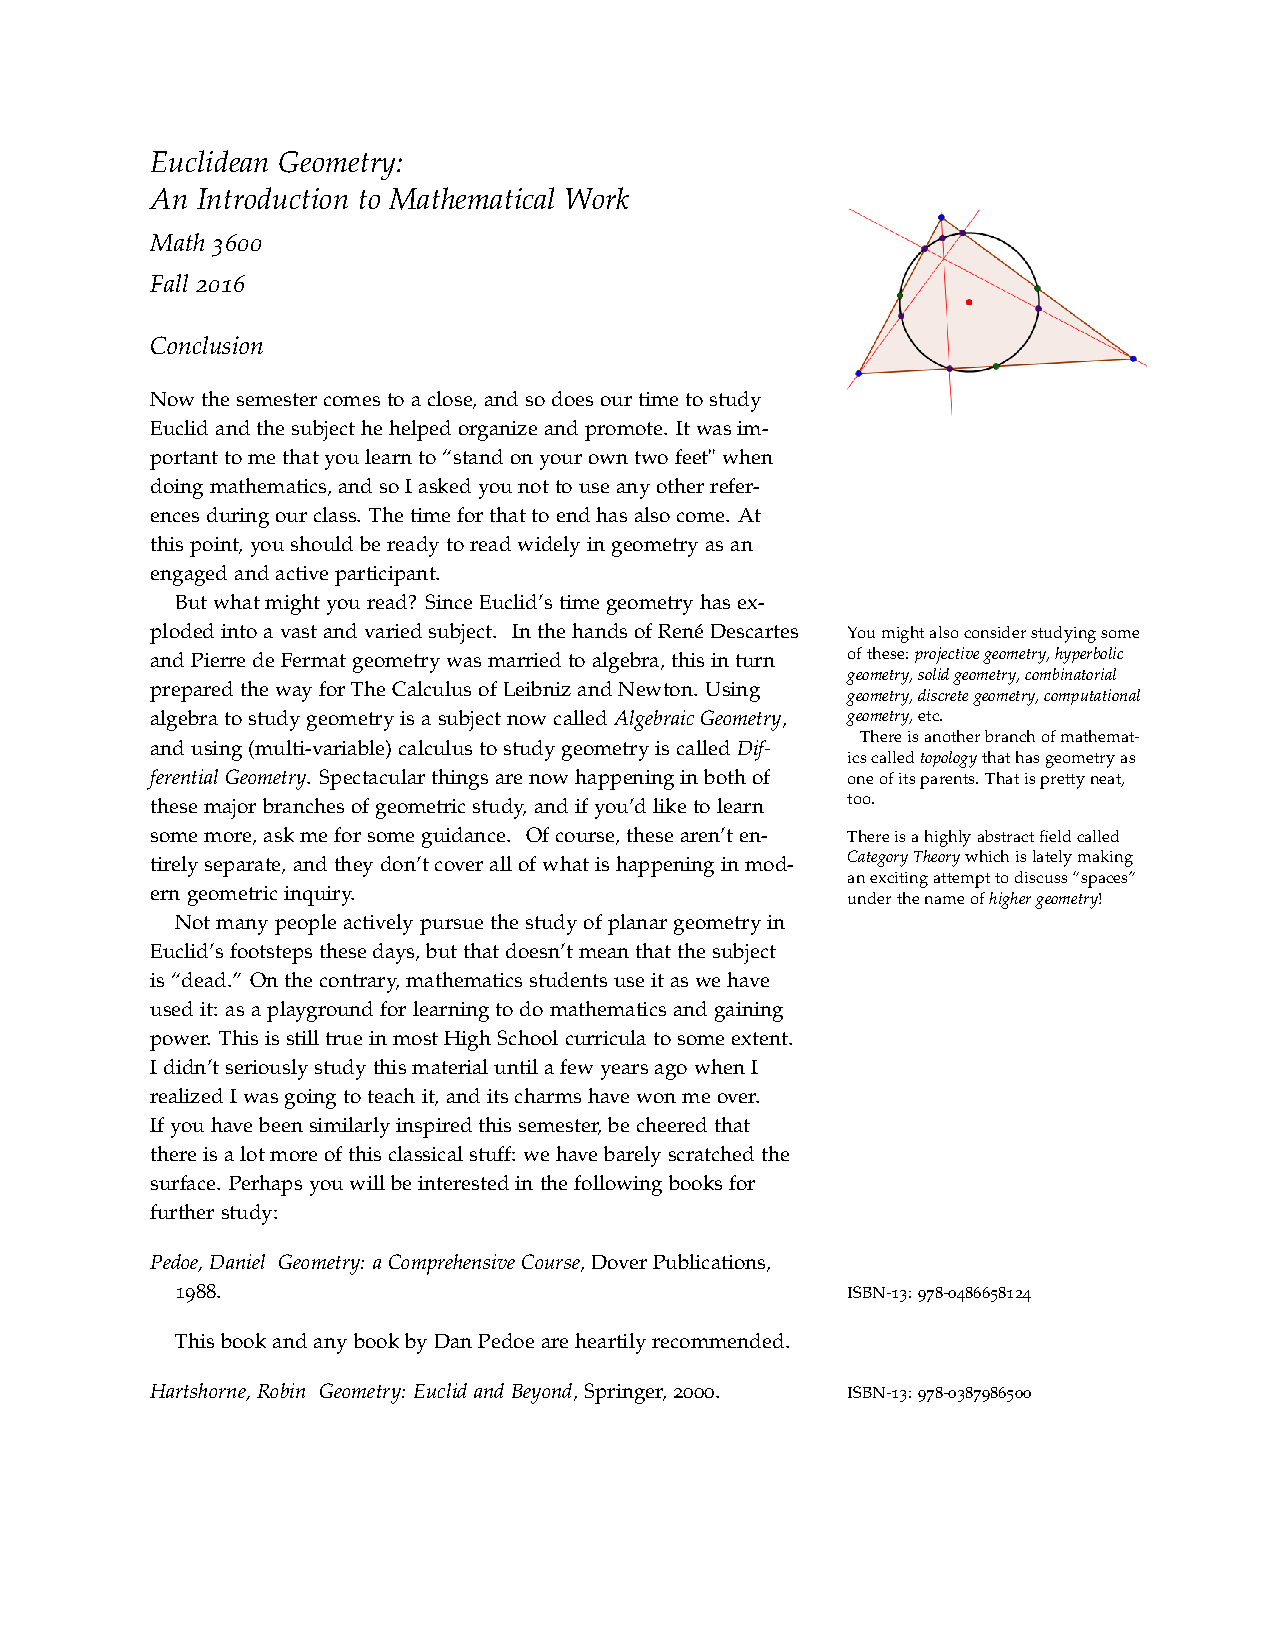
\includepdf[pages=-]{Conclusion.pdf}
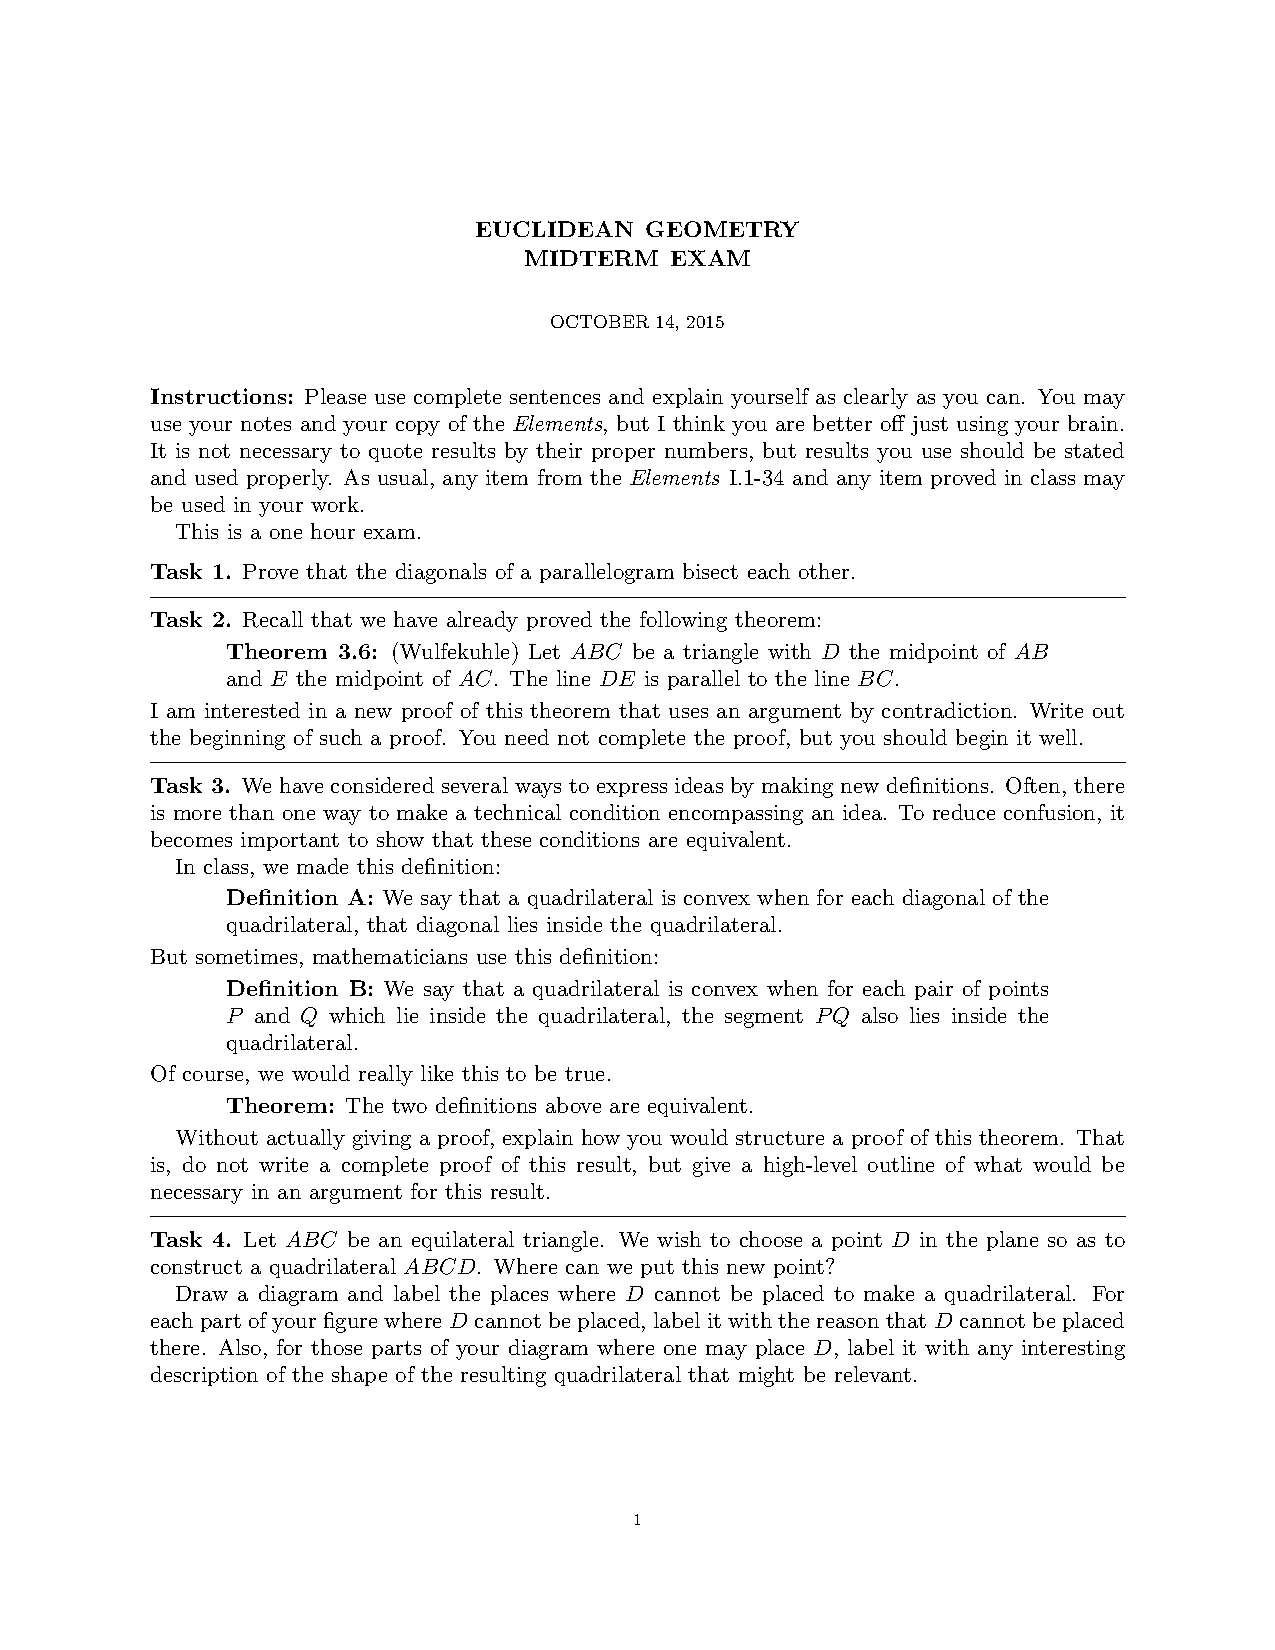
\includepdf[pages=-]{2015-Fa-EG-MidtermExam.pdf}
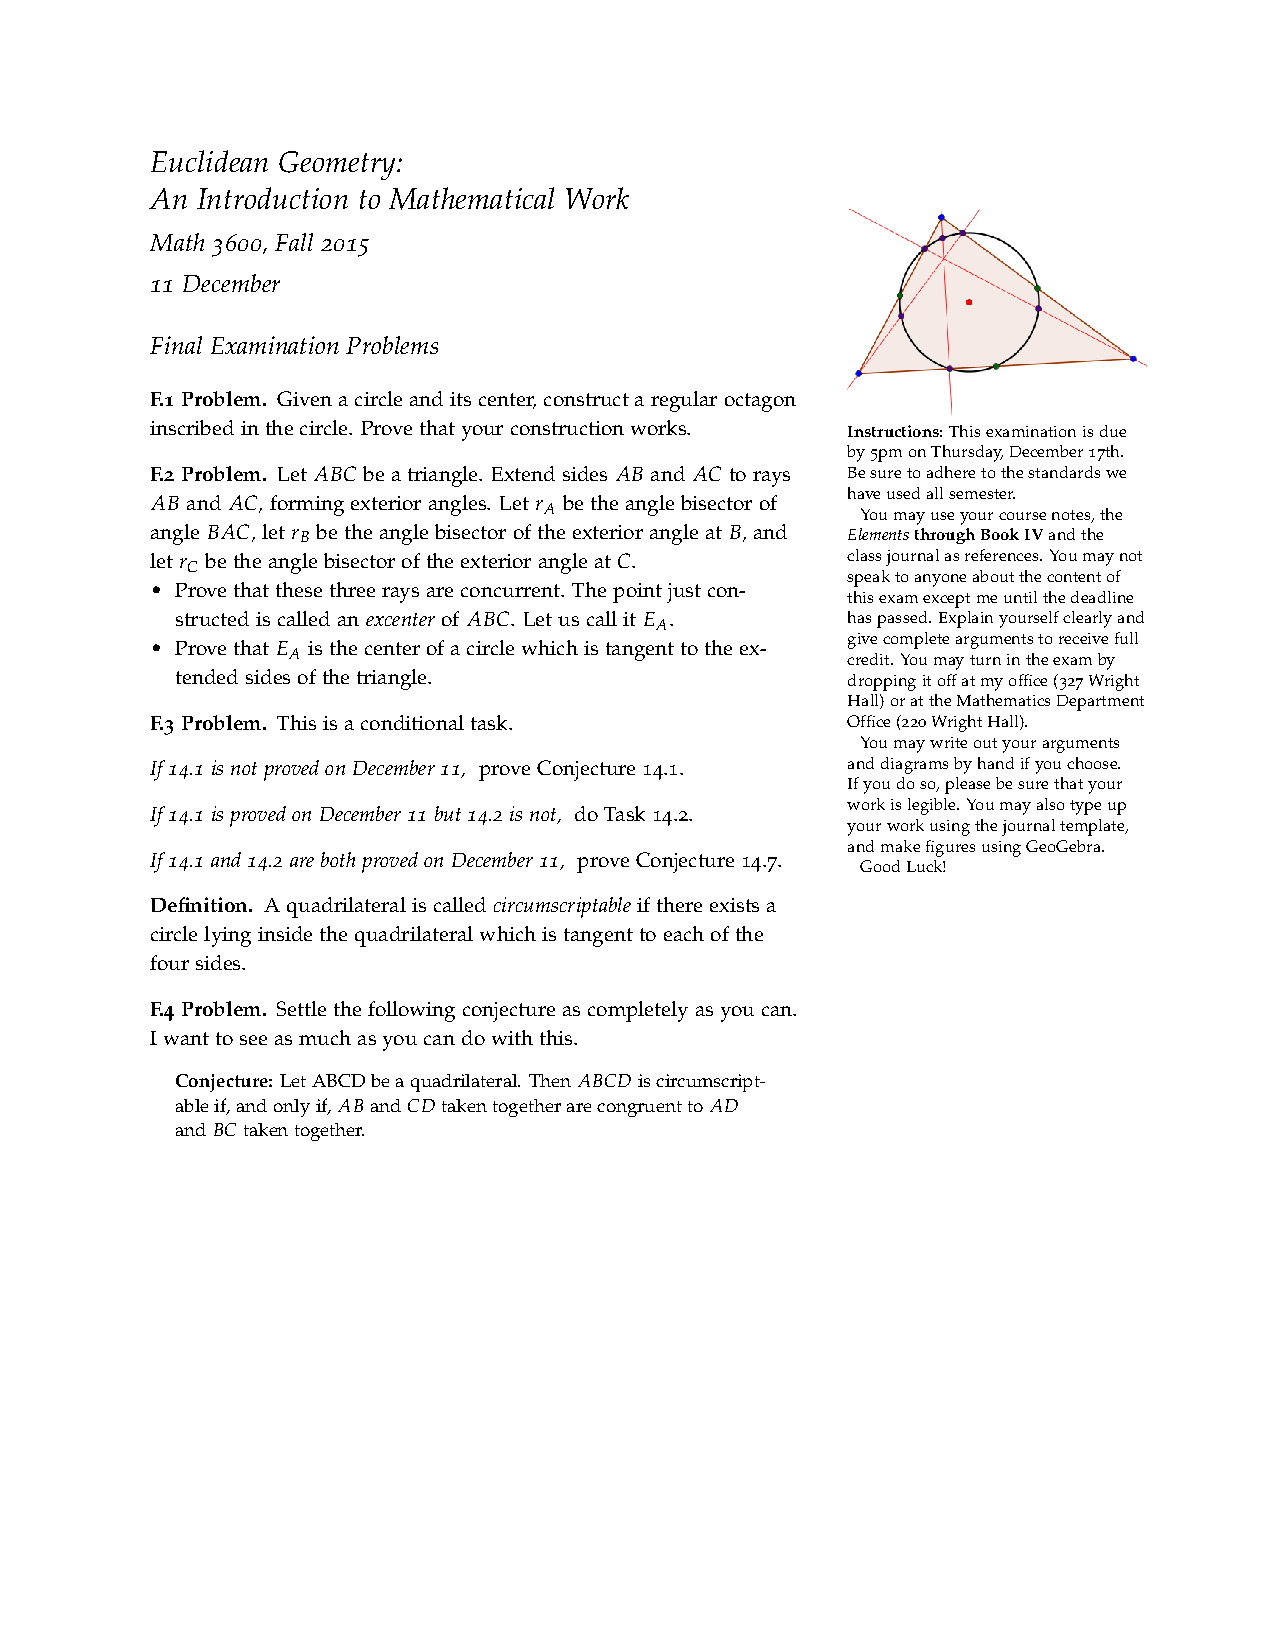
\includepdf[pages=-]{2015-Fa-EG-FinalExam.pdf}
\includepdf[pages=-]{the-standards.pdf}

\end{annotation}

\end{document}
